% !TeX encoding = UTF-8
% !TeX spellcheck = en_GB
% !TeX root = mythesis.tex
\chapter{Fractionally charged quasi-particle signature in microwave photons emission}

%Le projet de charge fractionnaires détectée par bruit RF


%\begin{enumerate}
%	\item Le set-up de mesure de bruit
%	\item Les calculs d'Ines-Safi
%	\item Les résultats de conductances et de bruit BF
%	\item Les résultats de bruit RF
%\end{enumerate}

\section{\texorpdfstring{...}{...}}

\subsection{\texorpdfstring{...}{...}}

% l'effet Hall classique donne des info sur porteurs de charge

\begin{figure}[hptb]
	\begin{center}
		\begin{tabular}{c c c c}
			(a) & & (b) & \\
			& 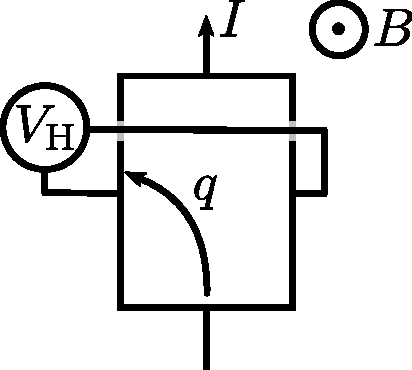
\includegraphics[width = 4 cm]{./chap2/effet_Hall_classique}
			& &
			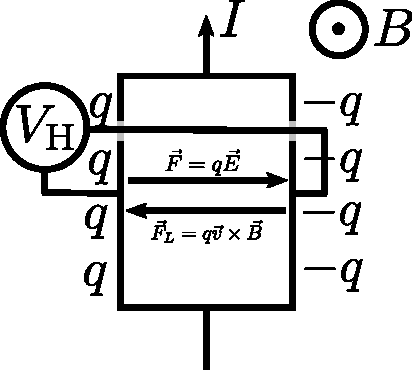
\includegraphics[width = 4 cm]{./chap2/effet_Hall_classique_bis} \\
		\end{tabular}
	\end{center}
	
	\caption{\textbf{title.}}
	\label{fig: effet Hall classique}
\end{figure}

The Hall effect is usually used to get charge $q$ and density $n$ of the charge carriers in a semiconductor.
The application of a perpendicular magnetic field $\vec{B}$ to a 2D conductor leads to the appearance of a voltage difference $V_{\mathrm{H}}$ perpendicularly to the current flow $I$.
The charges $q$ flowing through the semiconductor are deviated by the magnetic field with the Lorentz force $\vec{F}_L = q\vec{v}\times\vec{B}$.
As they are deviated perpendicularly to the current flow direction given by $q\vec{v}$, there is an accumulation of charges on the edges of the sample.
These charges on the edge of the sample create a voltage difference perpendicularly to the current, the Hall voltage $V_{\mathrm{H}}$.
The electrostatic force created by the Hall voltage balances the Lorentz force in the permanent regime, and one get the relation between the Hall voltage and the current \eqref{eq: Hall law} which introduces the Hall resistance \eqref{eq: Hall resistance}.

\begin{equation}
V_{\mathrm{H}} = R_{\mathrm{H}}I \label{eq: Hall law}
\end{equation}

\begin{equation}
R_{\mathrm{H}} = \frac{B}{nq} \label{eq: Hall resistance}
\end{equation}

with $n$ the surface density of charge, $q$ the charge of carriers, $B$ the magnetic field.
The Hall resistance is proportional to the magnetic field applied and the measurement of the proportionality coefficient gives the information of $q$ and $n$ on the charge carriers.
The 2D conductor used in this manuscript is an interface between two semiconductors of AlGaAs and GaAs, and the charge carrier are electrons of charge $q = -e$ given by Si donors whose number determines the surface density $n = 2.10^{11}$ cm$^{2}$.

\subsection{\texorpdfstring{...}{...}}

% si on va plus haut en champ on a effet Hall quantique entier, là on prend des infos avec le bruit BF et RF, on a fait ça pour régime entier


\begin{figure}[hptb]
	\begin{center}
		\begin{tabular}{c c c c}
			(a) & & (b) & \\
			& 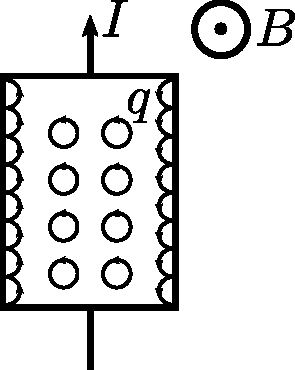
\includegraphics[width = 4 cm]{./chap2/effet_Hall_semi_classique} &
			& 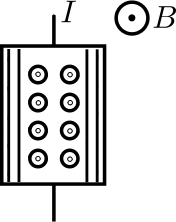
\includegraphics[width = 4 cm]{./chap2/effet_Hall_quantique}
		\end{tabular}
	\end{center}
	
	\caption{\textbf{title.} \textbf{(a)}  \textbf{(b)}}
	\label{fig: effet Hall quantique}
\end{figure}

\begin{figure}[hptb]
	\begin{center}
		\begin{tabular}{c c c c}
			(a) & & (b) & \\
			& 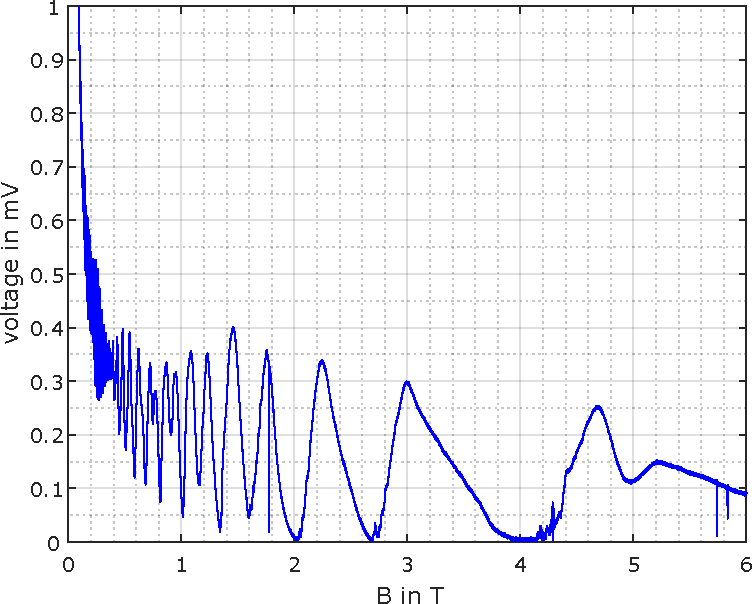
\includegraphics[width = 6.5 cm]{./chap2/backscattered_current} &
			& 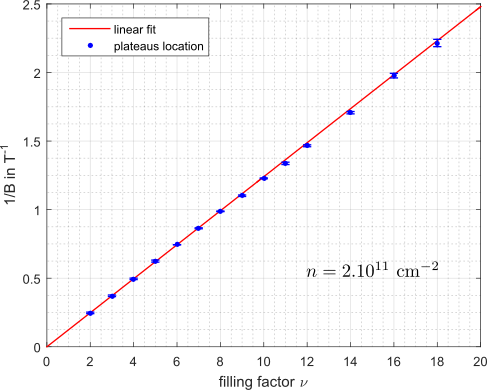
\includegraphics[width = 6.5 cm]{./chap2/B_vs_nu}
		\end{tabular}
	\end{center}
	
	\caption{\textbf{title.} \textbf{(a)}  \textbf{(b)}}
	\label{fig: backscattered current}
\end{figure}

For a high mobility 2D sample and at cold temperature one can observe that the Hall resistance is quantified for specific values which are fractions of the quantum of resistance \eqref{eq: quantum Hall resistance}, and the Hall resistance as a function of the magnetic field gives plateaus around corresponding magnetic field.

\begin{equation}
R_{\mathrm{H}} = \frac{1}{\nu}\times\frac{h}{e^{2}} \label{eq: quantum Hall resistance}
\end{equation}

with $\nu$ an integer number.
This quantification of the Hall resistance is the signature of the integer quantum Hall effect \cite{von1986quantized}.
In this regime, the electron system cannot be described by classical trajectories governed by Lorentz force, but is described by Landau levels.
The Landau levels are distributed in bands of discrete energies separated by the cyclotron pulsation $\hbar\omega_{c}$ and the Zeeman splitting $\hbar\omega_{z}$.
The cyclotron pulsation and the Zeeman splitting are proportional to the magnetic field $B$ which controls the number of bands below the Fermi energy.
This number of filled bands below the Fermi energy is the filling factor $\nu$ which is the integer number dividing the quantum of resistance in equation \eqref{eq: quantum Hall resistance}.
In this new regime, the electron transport is carried by $\nu$ states at the edge of the channel.
These states, called edge channel, are ballistic and chiral, so the longitudinal resistance of the sample is suppressed when the current is only carried by these edge channels, since the carriers are never backscattered.
In figure Fig. \ref{fig: backscattered current} panel (a), the backscattered voltage is measured as a function of the magnetic field $B$, and it reaches zero values.
The relation between the magnetic field and the filling factor \eqref{eq: B vs nu} is found by equations \eqref{eq: Hall resistance} and \eqref{eq: quantum Hall resistance}.

\begin{equation}
\frac{1}{B} = \frac{e}{nh}\nu \label{eq: B vs nu}
\end{equation}

By numbering the zeros of the panel (a), the panel (b) of figure Fig. \ref{fig: backscattered current} shows the inverse of the magnetic field as a function of the filling factor.
The data points are distributed on a linear curve as given by \eqref{eq: B vs nu}, and the slope of the fit gives the density of $n = 2.10^{11}$ cm$^{-2}$.
On the graph the filling factors 13, 15, and 17 are missing because for low magnetic field the Zeeman splitting is not big enough to separate Landau levels of different spin.

\subsubsection*{...}

%le bruit basse fréquence

In the quantum Hall effect, the electronic transport takes place on the edge channels.
To characterize the charge carriers in the edge channels, the low frequency noise can be used.
Schottky has demonstrated in \cite{schottky1918regarding} that the random partitioning of an electrical current generates a low frequency shot noise proportional to the charge of the carriers.


\subsubsection*{...}

\begin{figure}[hptb]
	\begin{center}
		\begin{tabular}{c c c c}
			(a) & & (b) & \\
			& 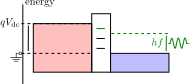
\includegraphics[width = 6.5 cm]{./chap2/noise_schematics_a} &
			& 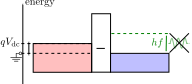
\includegraphics[width = 6.5 cm]{./chap2/noise_schematics_b}  
		\end{tabular}
	\end{center}
	
	\caption{\textbf{title.} \textbf{(a)}  \textbf{(b)} }
	\label{fig: principle schematics}
\end{figure}

Another method to determine the charge of carriers in the edge channel is to measure the high frequency noise.
The principle of this measurement is based on the Pauli exclusion principle and the quantification of the energy of microwave photons.
A DC voltage difference $V_{dc}$ is applied on the leads of a tunnel barrier, it shifts the Fermi level between the two leads of $qV_{\mathrm{dc}}$ with $q$ the charge of carriers.
This is drawn on figure Fig. \ref{fig: principle schematics} where the two leads are plotted in red and blue.
Charge carriers can tunnel through the tunnel barrier only between zero energy and $qV_{\mathrm{dc}}$, for energies higher than $qV_{\mathrm{dc}}$ there are no particles, for energies below the reference level all states are occupied on both leads so the Pauli exclusion principle avoid the tunnelling of charges.
As particles tunnels in an energy window of $qV_{\mathrm{dc}}$, the available energy in the system is bounded by $qV_{\mathrm{dc}}$.
The noise at frequency $f$ is the fluctuation of the signal at frequency $f$ in the microwave cable connected to the sample.
This signal can fluctuate only if microwave photons at frequency $f$ are emitted or absorbed by the cable, and the quantification of the energy of microwave photons set the energy exchange to be at least of $hf$ the energy of one photon.
In figure Fig. \ref{fig: principle schematics} the two panels shows two situations, in the panel (a) available energy $qV_{\mathrm{dc}}$ is higher than one microwave photon energy $hf$ so high frequency noise is generated, in the panel (b) $qV_{\mathrm{dc}}$ is below $hf$ so the high frequency noise is suppressed.
This transition between the regime without high frequency noise and with high frequency noise is obtained for a DC voltage $V_{dc} = \frac{hf}{q}$.
By measuring this transition, one gets a direct measurement of the charge $q$ since $V_{\mathrm{dc}}$ and $f$ are set by measurement instruments and not the properties of the sample such as the conduction of the tunnel barrier. 
This technique has been experimentally used in different conductors \cite{schoelkopf1997frequency,zakka2007experimental,gabelli2009high} revealing the elementary charge $q = e$ of electrons carrying the current in these systems.


\subsection{\texorpdfstring{...}{...}}

% et dans l'effet Hall quantique fractionnaire les porteurs ont la propriétée surprenante d'avoir une charge fractionnaire, ça été sondé avec le bruit BF, nous on fait ça avec du bruit RF en émission, c'est complémentaire aux mesures d'absorption de Kapfer.

\begin{figure}[hptb]
	\begin{center}
		\begin{tabular}{c}
			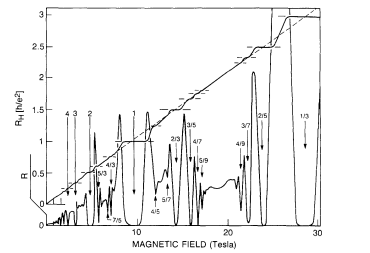
\includegraphics[width = 6.5 cm]{./chap2/fractional_Hall_resistance}
		\end{tabular}
	\end{center}
	
	\caption{\textbf{title.} }
	\label{fig: effet Hall quantique fractionnaire}
\end{figure}

The magnetic field can be increased such that the filling factor $\nu$ reaches values below one.
In this regime, the backscattered voltage drops also when the filling factor equals specific fractions such as $\dfrac{2}{3}$ or $\frac{1}{3}$, this characterizes the fractional quantum Hall effect.
The Hall resistance and the magnetic field at which this regime is reached is still determined by the fractional filling factor in equations \eqref{eq: quantum Hall resistance} and \eqref{eq: B vs nu}.
The strong electronic interactions change other properties of the electronic system such as the charge of carriers, indeed one can consider that the current is carried by quasiparticles of fractional charges.
These fractional charges have been measured through low frequency noise
by different experimental techniques.
The first techniques \cite{saminadayar1997observation,de1998direct,reznikov1999observation,bid2009shot,hashisaka2015shot} measure the low frequency noise generated by a quantum point contact when there is a DC voltage difference is applied at its inputs.
The output noise depends on both the conductance of the quantum point contact and on the charge of the carriers.
Another experimental technique realized in \cite{kapfer2019josephson,kapfer2018dynamic} still measures the output low frequency noise, but in addition to DC voltage difference applied to the inputs an extra RF sinus voltage is sent.
The added RF sinus voltage generates a photo-assisted shot noise from which the charge of carriers can be deduced as a function of the sinus frequency.
In the integer quantum Hall regime, the RF sinus of frequency $f$ modifies the electronic occupation by energy steps of size $hf$, these steps implies a slope variation of the noise when $qV_{\mathrm{dc}}$ reaches the same values, with $V_{\mathrm{dc}}$ the DC voltage applied.
The results of the article \cite{kapfer2019josephson} demonstrate that the same effect is obtained in the fractional regime with only $q$ equals a fractional charge.
This experiment investigates how a RF excitation is absorbed by the electronic system in the fractional regime.
This chapter presents a complementary experiment by measuring the emitted RF noise in the fractional regime.
As explained in the previous subsection and shown in \cite{schoelkopf1997frequency,zakka2007experimental,gabelli2009high}, one can deduce the charge of carriers by measuring the emitted high frequency noise.
This measurement of high frequency excitations also allows measuring the charge of carriers as a function of frequency and a DC voltage, without depending on the precise value of quantum point contact conductance.
When the excitations are electrons, the explanation of the results uses the Pauli exclusion principle, but in the fractional regime the excitations are anyons with a different statistic \cite{arovas1984fractional,halperin1984statistics,bartolomei2020fractional,nakamura2020direct}, so this chapter shows similar results without this principle \cite{haldane1991fractional}.


\section{\texorpdfstring{Experimental set-up}{Experimental set-up} \label{sec: Experimental set-up chap2}}

In this section the experimental techniques are detailed.
With a first part that describes the sample used and the low frequency characterizations and a second part that describes the high frequency noise measurement technique, whose experimental set-up is drawn in figure Fig. \ref{fig: le set-up chap2}.

\subsection{Low frequency set-up}

\begin{figure}
	\centering
	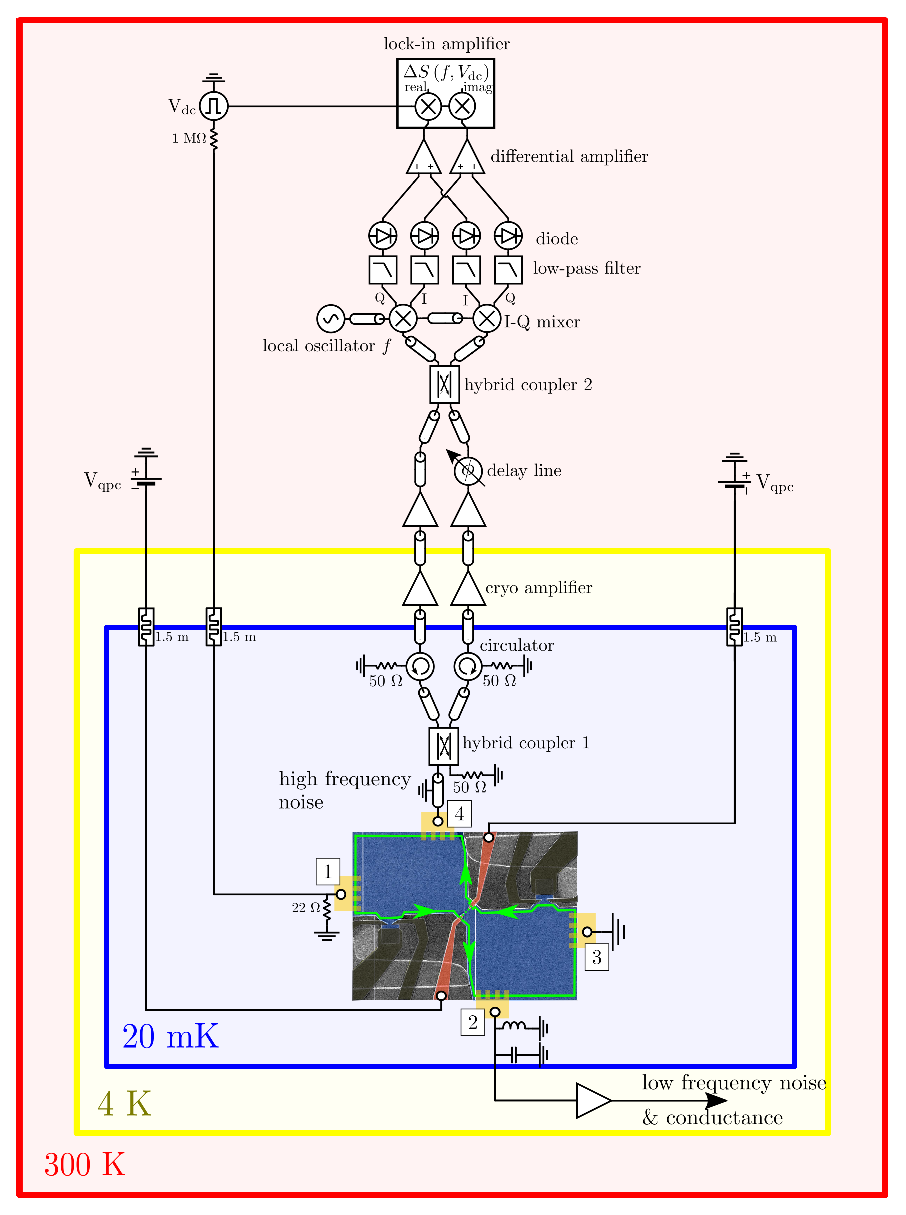
\includegraphics[width = 12cm]{./chap2/set-up_bruit_RF_pour_charge.eps}
	\caption{\textbf{Experimental set-up of high frequency noise measurement.} This schematic is separated in four regions: the red part at 300 K which is the exterior of the dilution fridge; the yellow part at 4K and the blue part at 20 mK which are inner stage of the dilution fridge; the sample SEM picture in false color which is the object studied. On the sample the 2D electron gas is coloured in blue, the quantum point contact gates in red, the Ohmic contacts are added in yellow, the outer edge-channel in green. DC voltage sources for gate voltages $V_{\mathrm{qpc}}$ are represented by a battery. The voltage source of DC bias $V_{\mathrm{dc}}$ is a very low frequency $\sim 230$ Hz squared voltage between 0 and $V_{\mathrm{dc}}$. The high frequency measurement set-up is detailed with the microwave Mach-Zehnder interferometer including amplifiers between the two hybrid couplers, the local oscillator with I-Q mixers and diodes to detect the noise power at a specific frequency, and the lock-in amplifier which demodulates the noise power generated by the bias voltage at the very low frequency of 230 Hz.  \label{fig: le set-up chap2}}
\end{figure}

The first measurements to characterize conductance and charge carriers are low frequency measurements.
The measurement lines used to perform them are minimally sketched on the figure Fig. \ref{fig: le set-up chap2} of this chapter, but it is fully drawn in the next chapter in figure Fig. \ref{fig: le set-up} and detailed in appendix in figure Fig. \ref{fig: output LF line}.
This organization is due to the fact that new measurements performed in this chapter are in the radio-frequency band, whereas the low frequency lines are used to perform new measurements in the next chapter.

\subsubsection*{DC voltage applied.}

\begin{figure}[hptb]
	\begin{center}
		\begin{tabular}{c c c c}
			(a) & & (b) & \\
			& 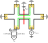
\includegraphics[width = 6.5 cm]{./chap2/Hall_bar_split_gate_open} &
			& 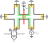
\includegraphics[width = 6.5 cm]{./chap2/Hall_bar_split_gate_close} \\
			(c) & & & \\
			& 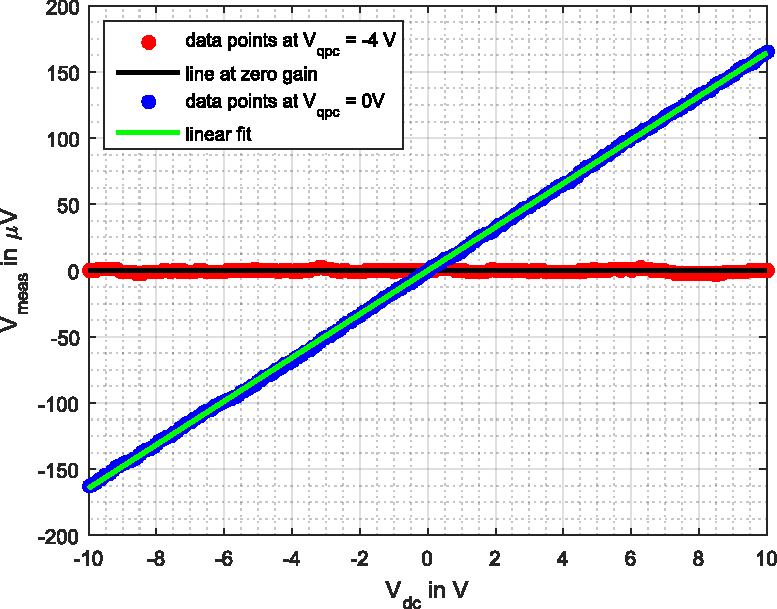
\includegraphics[width = 6.5 cm]{./chap2/DC_line_gain} &
			& 
			
		\end{tabular}
	\end{center}
	
	\caption{\textbf{Calibration at low temperature of DC voltage input line.} \textbf{(a)} Schematic of the Hall bar used to calibrate the attenuation of the bias voltage $V_{\mathrm{dc}}$ line. The limits of the 2D electron gas is delimited in black line, the Ohmic contacts are in yellow, the edge-channel in green, and the top gate in red. In this panel the voltage applied to the top gate is $V_{\mathrm{qpc}} = 0$ V, so the edge-channel is fully transmitted. \textbf{(b)} Same schematic as in previous panel but with a negative voltage applied to the gate $V_{\mathrm{qpc}} = -4$ V, this implies that the edge-channel is fully reflected by the top gate. \textbf{(c)} Voltage $V_{\mathrm{meas}}$ measured like on above panels as a function of bias voltage $V_{\mathrm{dc}}$. Data points in red are measured in panel (b) configuration, the measured voltages are independent of applied voltage $V_{\mathrm{dc}}$ and equal to zero as shown by the black line. Data points in blue are measured in the panel (a) case where, as the edge-channel is a ballistic conductor, the measured voltage equals the applied voltage in the edge-channel. The slope of the linear fit in green line is the measurement of the attenuation of the input line for $V_{\mathrm{dc}}$. This slope equals $1.64 \times 10^{-5}$.}
	\label{fig: DC line gain}
\end{figure}


The only sources used in this chapter are a DC voltage sources $V_{\mathrm{dc}}$ and $V_{\mathrm{qpc}}$, which are attenuated and thermalised.
The thermalisation of the lines occurs at the coldest stage thanks to a 1.5 m meander embedded in a copper powder filter.

One of the sources, carrying the voltage $V_{\mathrm{dc}}$, is connected to the Ohmic contact 1. 
It is attenuated by a voltage divider formed of a serial 1 M$\Omega$ resistor at room temperature and a parallel 22 $\Omega$ resistor at cold temperature contributing to the thermalisation of $V_{\mathrm{dc}}$.
As the DC voltage source used is limited by a 10 V range, this attenuation enables to work in a voltage range around 200 $\upmu$V at the sample level.
The 1 M$\Omega$ serial resistor is changed for a 0.68 M$\Omega$ resistor to reach at the sample a 300 $\upmu$V range and a 0.47 M$\Omega$ resistor to get a 500 $\upmu$V range.
To know precisely the voltage $V_{\mathrm{dc}}$ applied at the sample level, the voltage divider is calibrated at low temperature by replacing the sample by a Hall bar with a gate between the contacts, as in figure Fig. \ref{fig: DC line gain}.
For the calibration only, the voltage source is differential and two series resistors of total resistance $2\times 0.68$ M$\Omega$ contributes to the voltage divider.
When there is no voltage applied to the gate $V_{\mathrm{qpc}} = 0$ V, the edge channels are perfectly transmitted through the gate.
This implies that the DC voltage measured at the following Ohmic contact on the edge channel is the voltage at the sample level, as on the panel (a).
A linear fit of the measured voltage as a function of the applied voltage gives the voltage divider at low temperature, as given by the green line on the panel (c).
When the gate voltage  $V_{\mathrm{g}}$ is enough negative, one can check that the measured voltage is constant at zero, as shown by red points on the panel (c).
The DC voltage source shifts the chemical potential of one edge-channel through an Ohmic contact compared to the grounded opposite one as shown by the two horizontal green arrow in figure Fig. \ref{fig: le set-up chap2}.

The two opposite edge-channels meet at the central narrowing of the 2D electron gas in blue in the figure.
By applying a negative voltage $V_{\mathrm{qpc}}$ on the two red gates, one can adjust the electron transmission through a tunnel barrier, called quantum point contact, between the two edge-channels at the narrowing.
As the voltage range applied to the gates is about -1 V, there is no attenuation at cold temperature of the voltage applied $V_{\mathrm{qpc}}$, but they are still thermalised by meanders.

\subsubsection*{Conductance measurement.}

To measure the transmission of the central quantum point contact, a lock-in amplifier adds a small sine voltage to the DC source with a bias-tee, and measures the transmitted signal through the quantum point contact amplified by the noise measurement line.
The measured signal is proportional to the quantum point contact conductance at the bias voltage $V_{\mathrm{dc}}$ by identifying the plateaus of conductance as a function of $V_{\mathrm{qpc}}$, one can deduce the coefficient of proportionality.
On the schematics, only one edge-channel is represented, but depending on the magnetic field applied perpendicularly to the sample the number and the nature of the edge-channels change.
This can be probed by the quantum point contact conductance measurement and by the low frequency noise measurement.

\subsubsection*{Low frequency noise measurement.}

\begin{figure}[hptb]
	\begin{center}
		\begin{tabular}{c c c c}
			(a) & & (b) & \\
			& 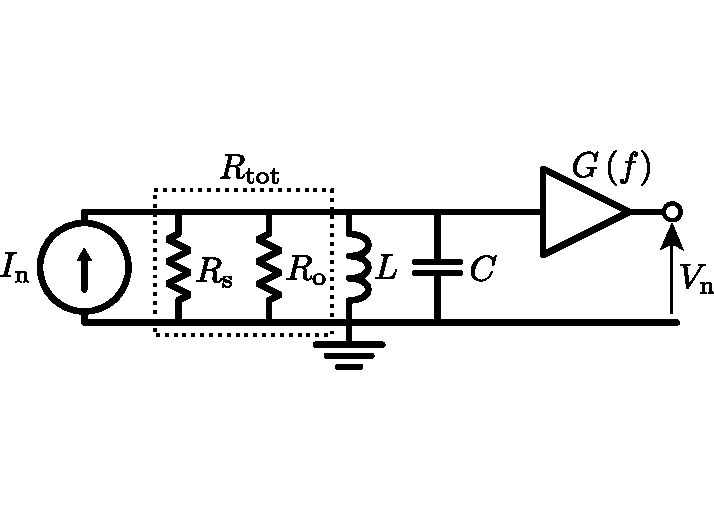
\includegraphics[width = 6.5 cm]{./chap2/gain_low_freq_noise} &
			& 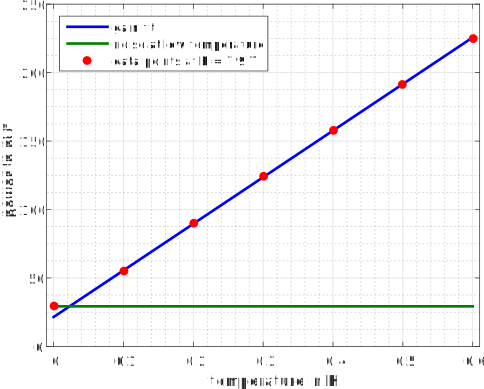
\includegraphics[width = 6.5 cm]{./chap2/temperature_calibration} \\
			(c) & & (d) & \\
			& 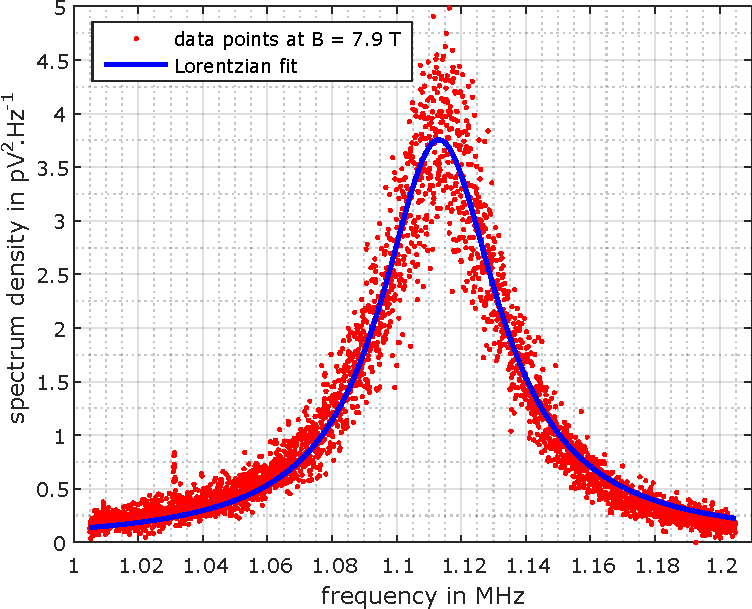
\includegraphics[width = 6.5 cm]{./chap2/noise_spectrum_nu_1} &
			& 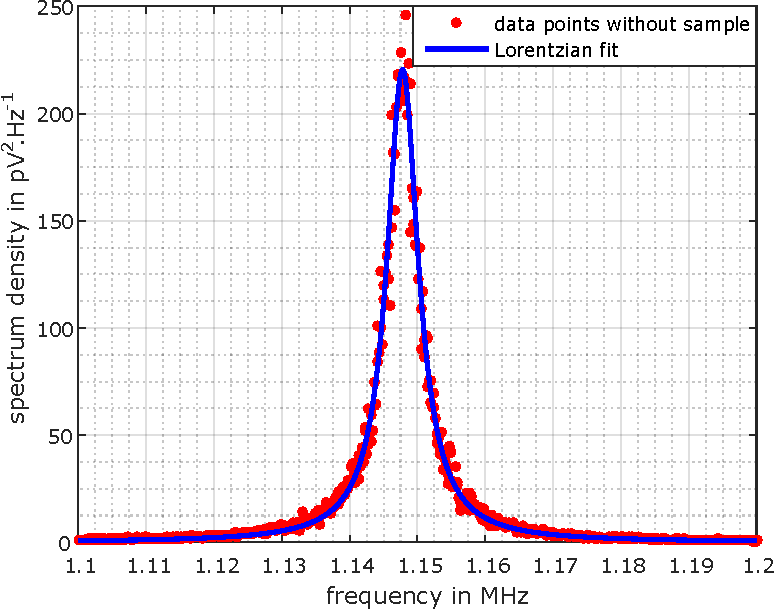
\includegraphics[width = 6.5 cm]{./chap2/noise_spectrum_open}
			
		\end{tabular}
	\end{center}
	
	\caption{\textbf{Low frequency noise measurement.} \textbf{(a)} The model of the measurement line is described by the drawn electronic circuit. The generated current noise $I_{\mathrm{n}}$ is distributed between the sample resistance $R_{\mathrm{s}}$, an added coil $L$, cables and amplifiers input capacitance $C$, a resistance $R_{\mathrm{o}}$ which models imperfection of the resonator. The voltage at their leads is amplified by amplifiers of gain $G$. \textbf{(b)} The power of the voltage noise $V_{\mathrm{n}}$ is plotted as a function of sample temperature. The resistance of the sample is fixed at $R_{\mathrm{s}} = \frac{h}{e^2}$ by the choice of the magnetic field $B = 7.9$ T. The data points at temperature above 100 mK are fitted by the blue line, its linear evolution is due to the increase of the thermal current noise. The lowest power measured at the lowest temperature is plotted by a red point at zero temperature and a green line. The crossing between the green and blue line gives the lowest temperature of electrons. \textbf{(c)} The measured power spectrum density is plotted as a function of frequency. It is the thermal noise of the sample of resistance $R_{\mathrm{s}} = \frac{h}{e^2}$ at a temperature of 600 mK. If the amplifiers gain is constant in the measurement bandwidth, the red data points are modelled by a Lorentzian resonance plotted in blue line. \textbf{(d)} The power spectrum density is measured without any sample connected.}
	\label{fig: low freq noise gain}
\end{figure}

The low frequency noise is measured at the Ohmic contact 2 see figure \ref{fig: le set-up chap2}.
First the core-less coil, which is connected in parallel, shifts with cable and amplifier input capacitances the measured noise at 1.1 MHz.
Then amplifiers and a vector spectrum analyser detects the noise spectrum at low frequency.
The calibration of the gain $G_{IV}^{2}$ of this measurement line is needed to get information on the system.
This gain is determined by three measurements plotted in figure Fig. \ref{fig: low freq noise gain}.
This determination procedure is explained in the following paragraphs with the example of a magnetic field of $B = 7.9$ T giving a filling factor $\nu = 1$.

The electrical model of these measurements is drawn on the panel (a), where a noise current source $I_{\mathrm{n}}$ is loaded by the sample resistance $R_{\mathrm{s}}$, the core-less coil $L$, the cable and amplifiers input capacitance $C$, and a resistor $R_{\mathrm{o}}$ taking into account the losses of the resonator.
The signal is then amplified with a gain $G$, to get the output voltage noise $V_{\mathrm{n}}$.
The first measurement consists of measuring with the vector spectrum analyser the power $P$ integrated on frequency of the voltage noise as a function of the temperature $T$ of the resistances.
The thermal excitations give a voltage noise spectrum density $S_{VV}$ proportional to the system temperature $T$ \eqref{eq: thermal spectrum density}:

\begin{equation}
S_{VV}\left(f\right) = \left|G\left(f\right)\right|^{2}\frac{4R_{\mathrm{tot}}k_{\mathrm{B}}T}{1+Q_{\mathrm{s}}^{2}\left(\frac{f}{f_{\mathrm{s}}}-\frac{f_{\mathrm{s}}}{f}\right)^{2}} \label{eq: thermal spectrum density}
\end{equation}

with $Q_{\mathrm{s}}$ and $f_{\mathrm{s}}$, the quality factor and resonance frequency of the set-up, and $R_{\mathrm{tot}}$ the total resistance formed by $R_{\mathrm{s}}$ and $R_{\mathrm{o}}$.

%On panel (b) the measured quantity as a function of temperature is the voltage noise power, which is the integral \eqref{eq: link power spectrum density} of the spectrum density.
Panel (b) represents measurements of the noise power $P$, which is the integral \eqref{eq: link power spectrum density} of the noise spectrum density, as a function of the temperature $T$.

\begin{equation}
P = \int_{f_{\mathrm{s}}-\frac{\Delta f_{\mathrm{s}}}{2}}^{f_{\mathrm{s}}+\frac{\Delta f_{\mathrm{s}}}{2}} S_{VV}\left(f\right)\mathrm{d}f \label{eq: link power spectrum density}
\end{equation}

On the measurement of figure Fig. \ref{fig: low freq noise gain} panel (b), we remark that the data points, in red points, can be fitted by a linear function $P = AT+B$, where the slope $A$ will be inversely proportional to the searched gain, and $B$ is the additional noise coming from the amplifiers.
The linear fit, in blue line, does not include the coldest point because we remark that below 40 mK the system temperature differs from the electrons temperature $T_{\mathrm{elec}} = ...$ mK.

The searched gain is the link between the measured power $P$ and the current noise spectrum $S_{II}$, given by \eqref{eq: link power current noise}, when the noise source is the shot noise generated at the quantum point contact.

\begin{equation}
P = \int_{f_{\mathrm{s}}-\frac{\Delta f_{\mathrm{s}}}{2}}^{f_{\mathrm{s}}+\frac{\Delta f_{\mathrm{s}}}{2}}\left|G\left(f\right)\right|^{2}\frac{R_{\mathrm{tot}}^{2}}{1+Q_{\mathrm{s}}^{2}\left(\frac{f}{f_{\mathrm{s}}}-\frac{f_{\mathrm{s}}}{f}\right)^{2}}S_{II}\mathrm{d}f \label{eq: link power current noise}
\end{equation}

At frequencies around 1 MHz, which are small compared to thermal excitations $\frac{k_{\mathrm{B}}T}{h} \sim 1$ GHz, the shot noise spectrum density does not depend on frequency, and thanks to the three above equations, the searched gain $G_{IV}^{2}$ is simply linked to the measured slope $A$ on the panel (b) by \eqref{eq: gain power to current noise}.

\begin{equation}
S_{II} = G_{IV}^{2}P \Rightarrow G_{IV}^{2} = \frac{4k_{\mathrm{B}}}{AR_{\mathrm{tot}}} \label{eq: gain power to current noise}
\end{equation}

In addition to the slope $A$, the gain $G_{IV}^{2}$ includes the total resistance of the sample resistance $R_{\mathrm{s}}$ in parallel with the open measurement chain resistance $R_{\mathrm{o}}$.
The sample resistance is known thanks to the quantization at each filling factor $\nu$ by $R_{\mathrm{s}} = \frac{h}{e^{2}\nu}$, but $R_{\mathrm{o}}$ has to be measured.
To do so we record the voltage noise spectrum density due to thermal noise with the sample connected in panel (c) and without the sample connected in panel (d).
From a Lorentzian fit of the resonance peak in the two measurements, we extract their quality factors and resonance frequencies, $Q_{\mathrm{s}}$ and $f_{\mathrm{s}}$ with sample, $Q_{\mathrm{0}}$ and $f_{\mathrm{0}}$ open loaded.
The resonance frequency is higher when the sample is removed because there are less cable and the capacitance decreases, but as the inductance remains constant we deduce the total resistance by equation \eqref{eq: link Rtot Rs}.

\begin{equation}
R_{\mathrm{tot}} = R_{\mathrm{s}}\left(1-\frac{Q_{\mathrm{s}}f_{\mathrm{s}}}{Q_{\mathrm{o}}f_{\mathrm{o}}}\right) \label{eq: link Rtot Rs}
\end{equation}

With this method we calibrate the gain $G_{IV}^{2}$ for all values of $\nu$ and we get for example $G_{IV}^{2} = ...$ S$^{2}$.Hz$^{-1}$.

\subsection{High frequency measurements}

The high frequency noise set-up is detailed in figure Fig. \ref{fig: le set-up chap2}, it is based on the set-up developed in \cite{parmentier2011high,parmentier2010short,engelbrecht1965wide,bisognin2019microwave}.
In this set-up the components to measure the noise at a chosen frequency are the I-Q mixers, low-pass filters, and the diodes.
The I-Q mixers multiply the signal by a local oscillator at the chosen frequency $f$, they perform a frequency translation in Fourier domain by shifting the signal around frequency $f$ towards DC signals.
The low-pass filters select the frequency bandwidth in which the noise is integrated, by suppressing all signals above their frequency cut-off.
The diodes square the noise and their dc signal outputs are proportional to the noise power.
The rest of the set-up, the amplifiers, the microwave Mach-Zehnder between the two hybrid couplers, and the modulation with the lock-in amplifier, enables to reach enough sensitivity to extract the signal from noise.
Indeed the order of magnitude of the measured signal around 7 GHz of partitioning elementary charges $e$ is $S_{\mathrm{meas.}} \sim e^{2}f \sim 1.10^{-29}$ A$^{2}.$Hz$^{-1}$.
This noise is compared to the thermal noises of the 50$\Omega$ impedance of the amplifiers at 4 K, which is around $S_{\mathrm{th.}} \sim 4Gk_{\mathrm{B}}T \sim 4.10^{-24}$ A$^{2}.$Hz$^{-1}$, and to the noise of the 50$\Omega$ resistor at the coldest part at 20 mK, which is of the order of $S_{\mathrm{th.}} \sim 2.10^{-26}$ A$^{2}.$Hz$^{-1}$.
So even at the lowest temperature, the thermal noise is three orders of magnitude above the measured signal.
The amplifiers amplify the signal above the room temperature thermal noise.
The microwave Mach-Zehnder reduces the amplifier noise by splitting it equally on the four diodes, so it is subtracted continuously by the differential amplifiers, whereas the signal is distributed only on the input "$+$" of the differential amplifiers.
Finally, the excitation modulation with a low frequency square function generator and the demodulation by the lock-in amplifier, enable to have enough stability to average until the measurement reaches enough sensitivity.
If one reads the measurement line schematics step by step, first the edge-channel is connected to a 50 $\Omega$ cable through an Ohmic contact.
This cable is connected to one input of hybrid coupler 1 and the other input is loaded with a 50 $\Omega$ resistor.
Let $a$ and $b$ be the signal at the two inputs, and $c$ and $d$ the signal at the outputs \eqref{eq: hybrid coupler 1}.

\begin{align}
	c & =  \frac{a+ib}{\sqrt{2}} \\
	d & =  \frac{ia+b}{\sqrt{2}} \label{eq: hybrid coupler 1}
\end{align}

The two amplifying chains are of gain $g_{1}$ and $g_{2}$, and they add the noises $\epsilon$, $\zeta$, the delay line balance the phase between the two chains by a phase $\theta$, this gives the signals after amplification $e$, $f$ \eqref{eq: amplifiers}.

\begin{align}
	e & =  g_{1}e^{i\theta}c+\epsilon \\
	f & =  g_{2}d+\zeta \label{eq: amplifiers}
\end{align}

The second hybrid coupler splits the amplifier noises $\epsilon$ and $\zeta$ between the two outputs and recombines the signal in its output $g$, $h$ \eqref{eq: hybrid coupler 2}.

\begin{align}
	g & =  \frac{e+if}{\sqrt{2}} \\
	h & =  \frac{ie+f}{\sqrt{2}} \label{eq: hybrid coupler 2}
\end{align}

The I-Q mixers separate the real and imaginary parts of the signal after shifting the frequency \eqref{eq: I-Q mixer}.
In the following equations, we keep only one pair of output ports of the I-Q mixers $g_{I}$ and $h_{Q}$.
The other pair $g_{Q}$ and $h_{I}$ gives analogue result for the other quadrature of the signal.

\begin{align}
	g_{I} & = \Re\left(g\right) \\
	h_{Q} & = \Im\left(h\right) \label{eq: I-Q mixer}
\end{align}

The low-pass filters and the diodes give in $k$ and $l$ the power of the noise \eqref{eq: diode}.
This power is integrated on the band defined by the low-pass filters, for these equations we assume this band to be negligible.

\begin{align}
	k & = \left<\left|g_{I}\right|^{2}\right> \\
	l & = \left<\left|h_{Q}\right|^{2}\right> \label{eq: diode}
\end{align}

The differential amplifiers subtract the two powers, and if one expresses the result $m$ as a function of the inputs it gives only an equation \eqref{eq: differential amplifier} as a function of first inputs $a$ and $b$. 

\begin{align}
	m & = k-l \\
	m & = g_{1}g_{2}\cos\left(\theta\right)\left(\left<\left|b_{Q}\right|^{2}\right>-\left<\left|a_{I}\right|^{2}\right>\right) \label{eq: differential amplifier}
\end{align}

The other pair of quadrature $g_{Q}$ and $h_{I}$ at equation \eqref{eq: I-Q mixer} gives a signal proportional to $\left<\left|a_{Q}\right|^{2}\right>$, the sum of these two signals gives the high frequency noise \eqref{eq: lien a et S}.

\begin{equation}
S\left(f,V_{\mathrm{dc}}\right) = \left<\left|a_{I}\right|^{2}\right> + \left<\left|a_{Q}\right|^{2}\right> \label{eq: lien a et S}
\end{equation}

The modulation suppresses the thermal noise $b$ and amplifier noise remaining from imperfections of the measurement set-up.
As the injected signal is modulated by a square function between zero voltage and $V_{\mathrm{dc}}$, the excess noise measured $\Delta S \left(f,V_{\mathrm{dc}}\right)$ is the difference \eqref{eq: excess finite freq noise} between the noise at applied voltages $V_{\mathrm{dc}}$ and 0.

\begin{equation}
\Delta S \left(f,V_{\mathrm{dc}}\right) = S \left(f,V_{dc}\right)-S \left(f,0\right) \label{eq: excess finite freq noise}
\end{equation}

The set-up presented here enables to access both low frequency noise $S\left(f=0,V_{\mathrm{dc}}\right)$ and high frequency noise $S\left(f,V_{\mathrm{dc}}\right)$ generated by a biased quantum point contact.

\section{\texorpdfstring{Charge determination by high frequency noise measurements}{Charge determination by high frequency noise measurements}}

This section presents the results given by the measurement set-up presented above.
The measurements are performed for different magnetic field applied to the sample and measurement frequencies.
All the measurements for different parameters are detailed, then they are summarized to compare their dependence in charge of carriers and frequency.

\subsection{Integer quantum Hall effect regime}

In the integer quantum Hall effect, the electrical current propagates along a number of edge-channels defined by the filling factor $\nu$.
By applying a magnetic field of $B = 4$ T or a magnetic field of $B = 2.6$ T perpendicularly to the 2D electron gas, we set the filling factor of the sample at 2 or 3, due to its density $n$, because $\nu = \frac{hn}{eB}$.
At these filling factors, the charges carrying the currents are electrons of elementary charge $-e$.
The measurements at these filling factor enable to validate the working principle of the measurement.

\subsubsection*{One measurement of the elementary charge at $\nu=2$.}

\begin{figure}[hptb]
	\begin{center}
		\begin{tabular}{c c c c}
			(a) & & (b) & \\
			& 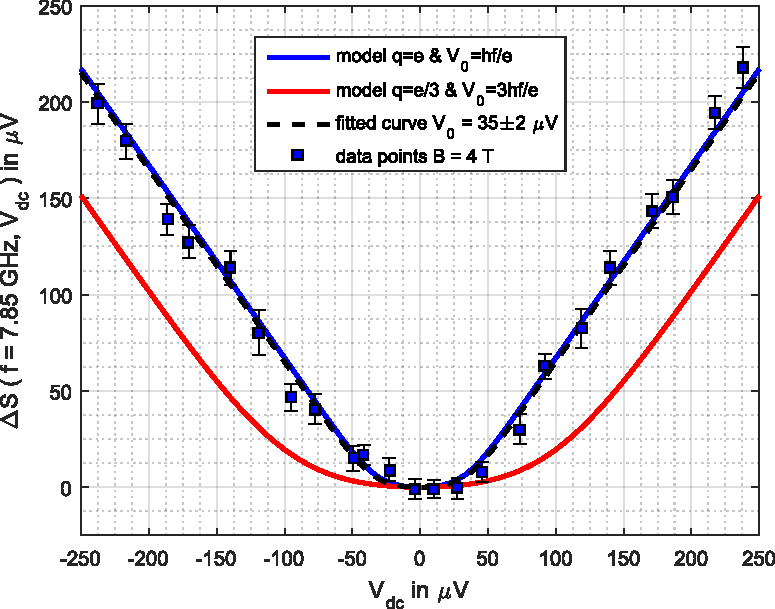
\includegraphics[width = 6.5 cm]{./chap2/nu_2_RF_noise_vs_Vdc_at_7_85GHz} &
			& 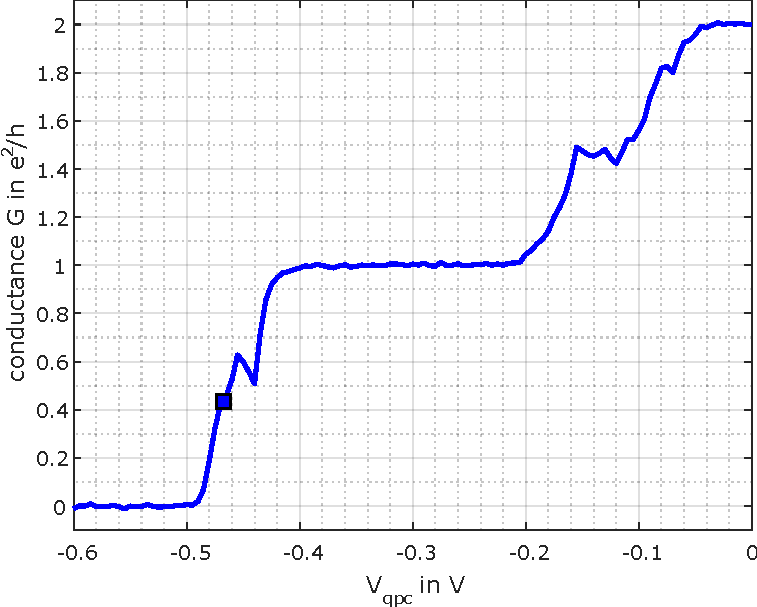
\includegraphics[width = 6.25 cm]{./chap2/qpc_step_nu_2}
		\end{tabular}
	\end{center}
	
	\caption{\textbf{High frequency noise measurement at integer filling factor $\nu = 2$.} \textbf{(a)} Data blue square points are measured at a frequency of 7.85 GHz as a function of bias voltage. The data points are consistent with the model of charge $q = e$ in blue line. The model of charge $q = \frac{e}{3}$ in red line is well separated from data points. The dashed line is the result of the model with the threshold voltage of noise emission $V_{0}$ let as a free fitting parameter. \textbf{(b)} Conductance measurement as a function of gate voltage $V_{\mathrm{qpc}}$ at zero bias $V_{\mathrm{dc}} = 0$ V. The two steps of the same amplitude of the blue line confirm the filling factor $\nu = 2$. The square point labels the gate voltage and transmission of the quantum point contact at which the high frequency noise is measured.}
	\label{fig: RF charac at 2}
\end{figure}

At the filling factor $\nu = 2$, the quantum point contact transmission is adjusted such that the inner edge-channel is totally reflected and the outer edge-channel is half transmitting.
%The local oscillator sets the measurement frequency at $f = 7.85$ GHz, in order that the no noise plateau without excess noise is larger in voltage than the thermal blurring with an electronic temperature $T_{\mathrm{elec}} = 50$ mK, $hf \gg k_{\mathrm{B}}T_{\mathrm{elec}}$.
The local oscillator sets the measurement frequency at $f = 7.85$ GHz, in order that the energy associated is bigger than the electronic temperature $hf \gg k_{\mathrm{B}}T_{\mathrm{elec}}$.
In the measurements of figure Fig. \ref{fig: RF charac at 2}, this implies that for low bias voltage $eV_{\mathrm{dc}} < hf$ neither the bias voltage nor the thermal excitations have enough energy to generate noise at frequency $f$, and the figure shows a plateau at $\Delta S\left(f,V_{\mathrm{dc}}\right) = 0$ $\upmu$V at low voltages.
%In measurements the rounding around the corners between the no noise plateau and the noise linear increase is dominated by the frequency bandwidth chosen with a cut-off frequency of low pass-filter at $\Delta f = 1.5$ GHz, because it correspond to a bigger energy than the temperature $h\Delta f > k_{\mathrm{B}}T_{\mathrm{elec}}$.
The frequency bandwidth is chosen with a cut-off frequency of low pass-filter at $\Delta f = 1.5$ GHz, as it corresponds to a bigger energy than the temperature $h\Delta f > k_{\mathrm{B}}T_{\mathrm{elec}}$ , it determines the rounding between the noise plateau at $\Delta S\left(f,V_{\mathrm{dc}}\right) = 0$ $\upmu$V and the linear increase of the noise.
The DC voltage applied belongs to a 200 $\upmu$V range, which is much greater than the expected threshold voltage $\frac{hf}{e} = 32 \upmu$V.
For voltages above this threshold data points plotted as blue squares in figure Fig. \ref{fig: RF charac at 2}, follow a linear curve.
The values of the noise are given by the voltages read at the lock-in amplifier, and in the figures the measurements are divided by one gain for each curves such that the slope of the linear part are $\pm1$ so $\Delta S \left(f,V_{\mathrm{dc}}\right) = \left|V_{\mathrm{dc}} \pm V_{0}\right|$ and the noise is expressed in $\upmu$V.
On the same graph Fig. \ref{fig: RF charac at 2} is plotted in blue line the expected curve for a non-interacting model \cite{blanter2000shot,martin2005course} of charge $e$, with an effective temperature $T_{\mathrm{elec}}$ due to the measurement bandwidth.
This model is expressed by the equation \eqref{eq: RF noise charge e}.

\begin{equation}
\Delta S \left(f,V_{\mathrm{dc}}\right) = \frac{1}{2}\left(V_{\mathrm{dc}}+\frac{hf}{q}\right)\coth\left(\frac{qV_{\mathrm{dc}}+hf}{2k_{\mathrm{B}}T_{\mathrm{elec}}}\right)+\frac{1}{2}\left(V_{\mathrm{dc}}-\frac{hf}{q}\right)\coth\left(\frac{qV_{\mathrm{dc}}-hf}{2k_{\mathrm{B}}T_{\mathrm{elec}}}\right)-\frac{hf}{q}\coth\left(\frac{hf}{2k_{\mathrm{B}}T_{\mathrm{elec}}}\right) \label{eq: RF noise charge e}
\end{equation}

with $q = e$.
The measured data points are consistent with this model. For the same non-interacting model with a fractional charge $e^{\star} = \frac{e}{3}$, the equation \eqref{eq: RF noise charge e} is unchanged except for the charge $q$ which is replaced by the fractional charge $e^{\star}$.
The red line plotted on the figure is given by this model with a fractional charge.
The data points with the sizes of their errobars allow excluding this last model, which demonstrates the ability of the technique to distinguish between situations with charge $e$ and $e^{\star}$.
The parameter which differentiates in this measurement the two models is the threshold voltage between the regime where the excess noise is constant at zero and its linear dependence as a function of voltage.
This threshold voltage, noted $V_{0}$, is linked to the excitation charges $q$ by the equation \eqref{eq: Josephson relation}, called the Josephson relation because it is the same equation as in a superconducting Josephson junction.

\begin{equation}
V_{0} = \frac{hf}{q} \label{eq: Josephson relation}
\end{equation}

To determine the measured value of $V_{0}$, the data points are fitted by the equation \eqref{eq: fit RF noise} with the parameter $V_{0}$ let as a free parameter.

\begin{equation}
\Delta S \left(f,V_{\mathrm{dc}}\right) = \frac{1}{2}\left(V_{\mathrm{dc}}+V_{0}\right)\coth\left(q\frac{V_{\mathrm{dc}}+V_{0}}{2k_{\mathrm{B}}T_{\mathrm{elec}}}\right)+\frac{1}{2}\left(V_{\mathrm{dc}}-V_{0}\right)\coth\left(q\frac{V_{\mathrm{dc}}-V_{0}}{2k_{\mathrm{B}}T_{\mathrm{elec}}}\right)-V_{0}\coth\left(\frac{qV_{0}}{2k_{\mathrm{B}}T_{\mathrm{elec}}}\right) \label{eq: fit RF noise}
\end{equation}

The resulting trace from this fitting procedure is represented as dashed black line in figure Fig. \ref{fig: RF charac at 2} and gives a value of $V_{0} = 35 \pm 2$ $\upmu$V.

\subsubsection*{Measurements for different frequencies at $\nu=3$.}

\begin{figure}[hptb]
	\begin{center}
		\begin{tabular}{c c c c}
			(a) & & (b) & \\
			& 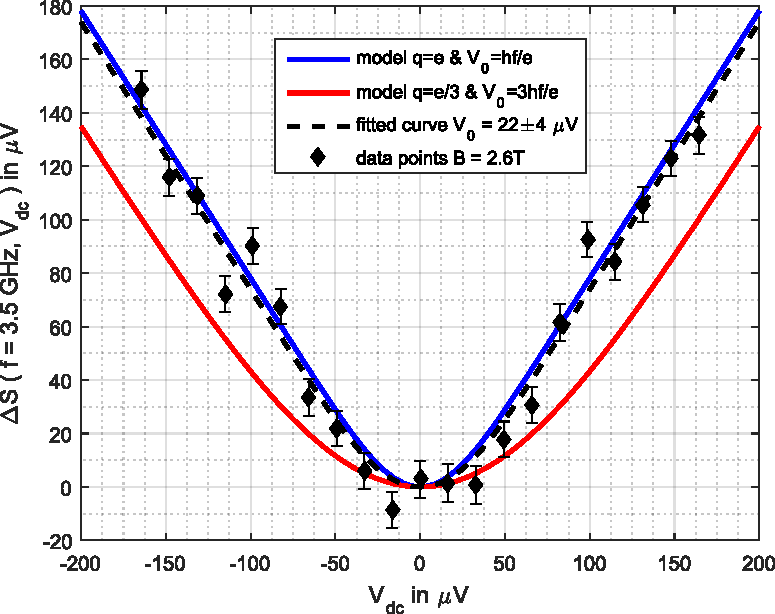
\includegraphics[width = 6.5 cm]{./chap2/nu_3_RF_noise_vs_Vdc_at_3_5GHz} &
			& 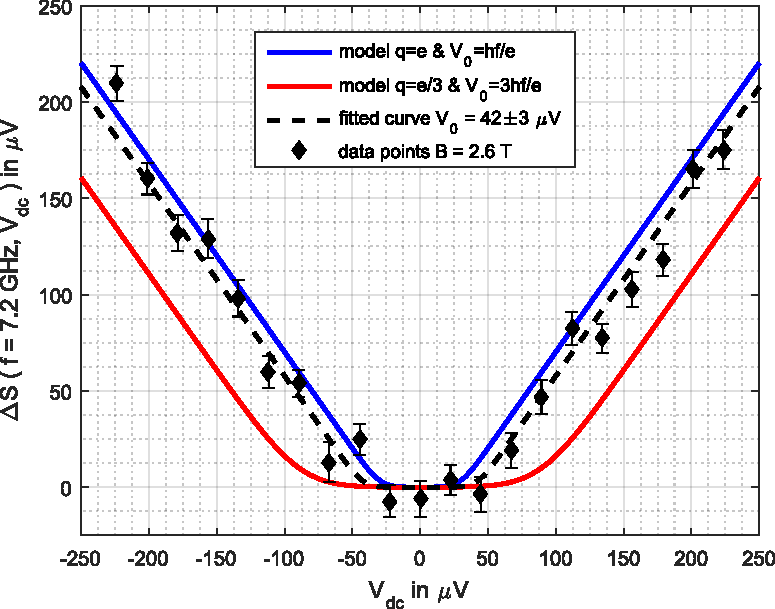
\includegraphics[width = 6.5 cm]{./chap2/nu_3_RF_noise_vs_Vdc_at_7_2GHz} \\
			(c) & & (d) & \\
			& 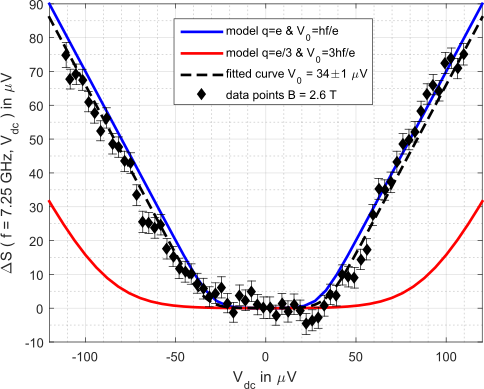
\includegraphics[width = 6.5 cm]{./chap2/nu_3_RF_noise_vs_Vdc_at_7_25GHz} &
			& 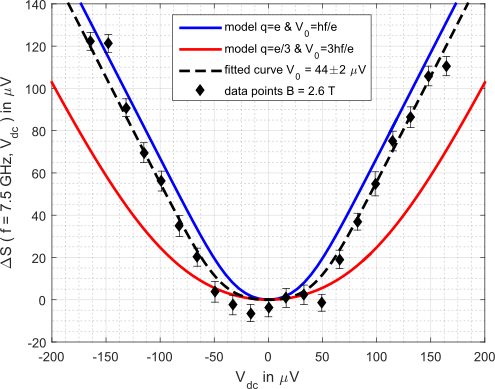
\includegraphics[width = 6.5 cm]{./chap2/nu_3_RF_noise_vs_Vdc_at_7_5GHz} \\
			(e) & & (f) & \\
			& 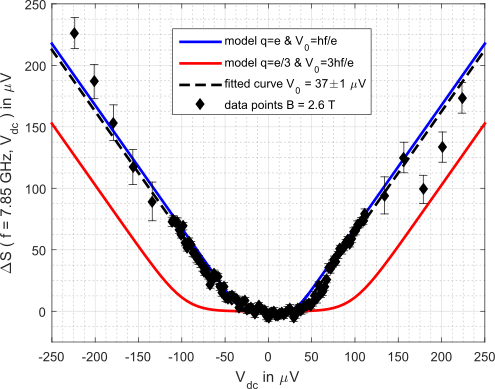
\includegraphics[width = 6.5 cm]{./chap2/nu_3_RF_noise_vs_Vdc_at_7_85GHz} &
			& 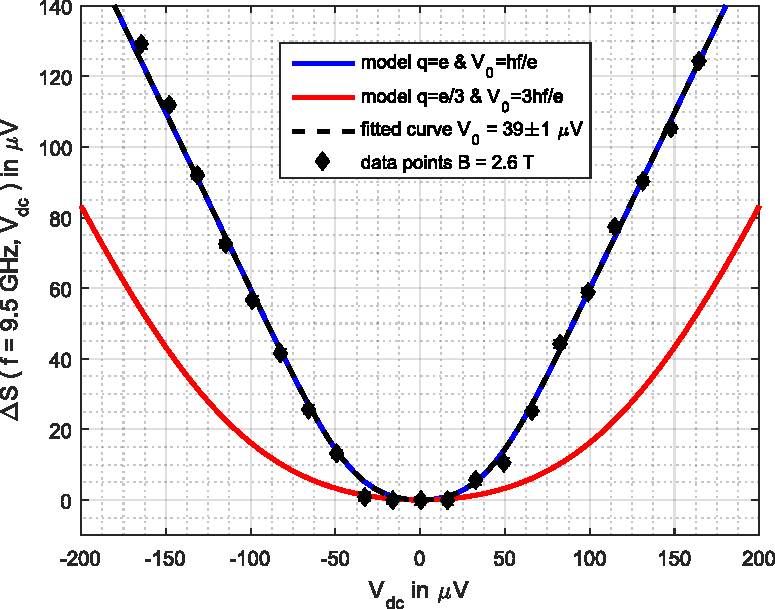
\includegraphics[width = 6.5 cm]{./chap2/nu_3_RF_noise_vs_Vdc_at_9_5GHz}
		\end{tabular}
	\end{center}
	
	\caption{\textbf{High frequency noise measurement for frequencies between $f = 3.5$ GHz and $f = 9.5$ GHz at filling factor $\nu = 3$.} The data points are plotted in black diamonds for this filling factor. For all curves integer charge $q = e$ models are still in blue lines, fractional charge models are still in red lines, and fitted lines in dashed lines. The data points and fitted curves agree with the model $q=e$ in all panels. The different parameter between panels is the increasing of the measurement frequency $f$ with \textbf{(a)} $f = 3.5$ GHz \textbf{(b)} $f = 7.2$ GHz \textbf{(c)} $f = 7.25$ GHz \textbf{(d)} $f = 7.5$ GHz \textbf{(e)} $f = 7.85$ GHz \textbf{(f)} $f = 9.5$ GHz.}
	\label{fig: RF charac at 3}
\end{figure}

In the relation \eqref{eq: Josephson relation}, $V_{0}$ remains constant between filling factors $\nu = 2$ and $\nu = 3$, because the current is still carried by electrons of charge $q = e$.
The other term is the frequency $f$ at which one measure the noise $\Delta S \left(f,V_{\mathrm{dc}}\right)$.
In this paragraph, we choose a filling factor $\nu = 3$ by applying a magnetic field $B = 2.6$ T, and the frequency $f$ has been changed first at $f = 3.5$ GHz, then around $f = 7.5$ GHz, finally at $f = 9.5$ GHz.
The measurement results are displayed in figure Fig. \ref{fig: RF charac at 3} with one panel for each frequency.
The data points at $\nu = 3$ are plotted in black diamonds, and the colour codes are conserved for the models, with blue lines corresponding to equation \eqref{eq: RF noise charge e}, red lines to the same equation with fractional charge $q = e^{\star}$, and dashed lines to a fit with the parameter $V_{0}$.
Among the different panels the range of the $V_{\mathrm{dc}}$ values change because as explained in the section \ref{sec: Experimental set-up chap2}, the voltage divider used to applied $V_{\mathrm{dc}}$ is changed.
The round shape at the threshold voltage $V_{0}$ has also not the same width between the graphs, because the bandwidth of noise integration varies by the changes of the low-pass filters, this is taken into account by selecting the correspondent $T_{\mathrm{elec}}$ in the models. 
The values of noise $\Delta S \left(f,V_{\mathrm{dc}}\right)$ are still divided by their slopes in the linear part of each curve, so they are expressed in $\upmu$V with a gain of 1.
On all panels the data points are close to the blue line of charge $q = e$ in comparison with their error-bars, and they are far from the red line of charge $q = e^{\star}$.
In the same way the fitted curve in dashed line is much closer to the blue than the red line, so the current is still carried by electrons at $\nu = 3$.
The results $V_{0}$ from the fits of each graph increase with frequency overall measurements from $V_{0} = 22 \pm 4$ $\upmu$V at $f = 3.5$ GHz in the panel (a) to $V_{0} = 39 \pm 1$ $\upmu$V at $f = 9.5$ GHz in the panel (f).
This increase is consistent with the frequency dependence of relation \eqref{eq: Josephson relation}, where the threshold voltage is proportional to the frequency $f$.

\subsection{Fractional quantum Hall effect regime}

The experimental method has been validated with the above measurement in the integer quantum Hall regime, so it can be used to investigate the fractional quantum Hall regime.

\subsubsection*{First fractional charges measurement at $\nu = \frac{2}{3}$.}

The first technique to reach the fractional regime is to increase the magnetic field until the filling factor of the sample is fractional.
In the following results the filling factor at which we stop is $\nu = \frac{2}{3}$ at a magnetic field of $B = 12$ T.
We did not reach $\nu = \frac{1}{3}$, which is a better defined fractional state, because it would have required, with the used samples of charge carrier density of $n = \nu\frac{eB}{h} \sim 2.10^{11}$ cm$^{-2}$, to apply a twice stronger magnetic field of $B = 24$ T well above the capacity of our system.

\paragraph*{Low frequency characterization.}

\begin{figure}[hptb]
	\begin{center}
		\begin{tabular}{c c c c}
			(a) & & (b) & \\
			& 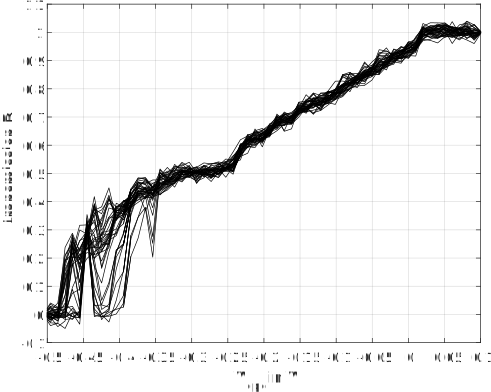
\includegraphics[width = 6.5 cm]{./chap2/nu_2_3_D_vs_Vqpc_for_several_Vdc} &
			& 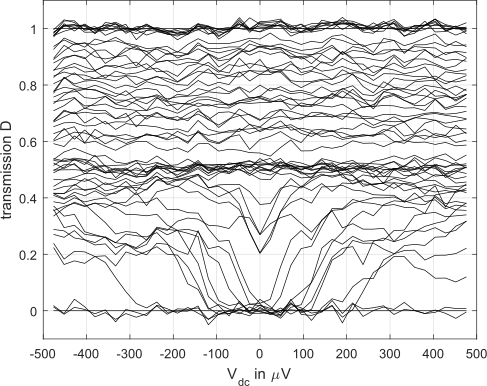
\includegraphics[width = 6.5 cm]{./chap2/nu_2_3_D_vs_Vdc_for_several_Vqpc} \\
			(c) & & (d) & \\
			& 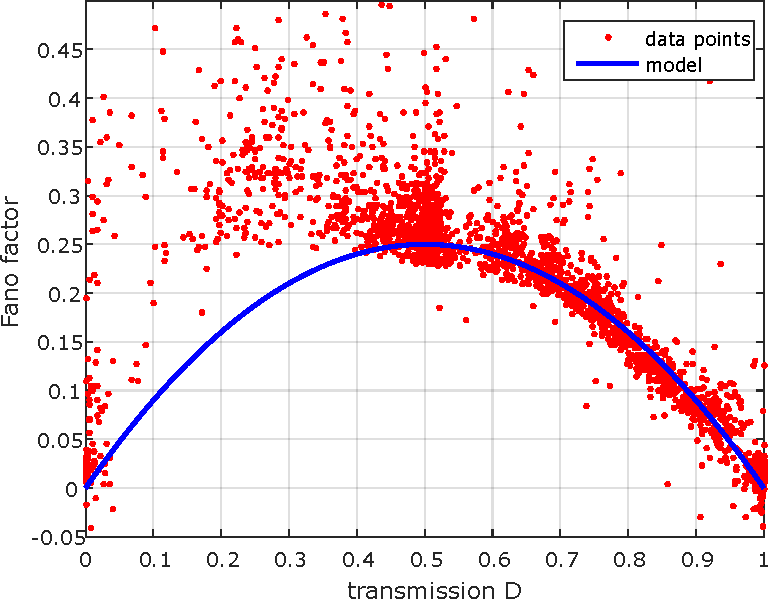
\includegraphics[width = 6.5 cm]{./chap2/nu_2_3_noise_vs_D_for_several_Vdc} &
			& 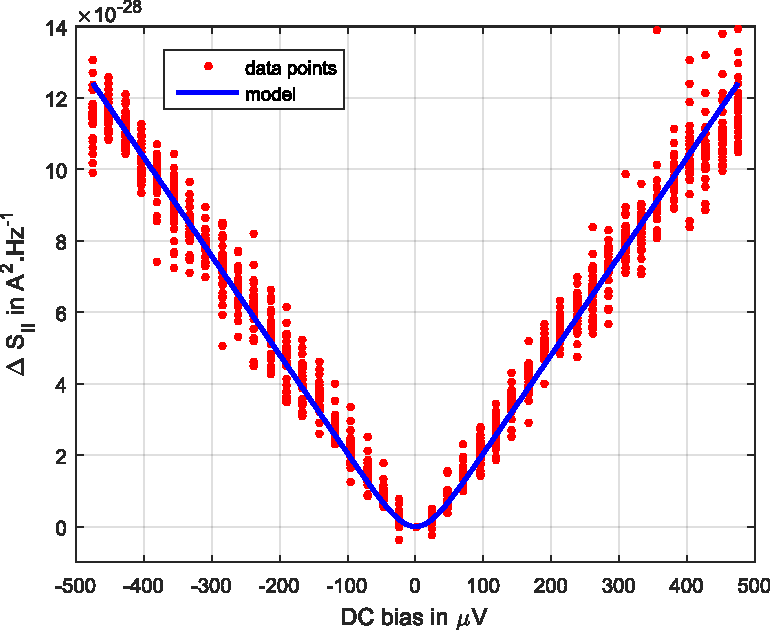
\includegraphics[width = 6.5 cm]{./chap2/nu_2_3_noise_vs_Vdc_for_D_0_4_0_9}
			
		\end{tabular}
	\end{center}
	
	\caption{\textbf{Conductance and low frequency noise measurement at fractional filling factor $\nu = \frac{2}{3}$.} Panels (a) and (b) are conductance measurements as a function of gate voltages $V_{\mathrm{qpc}}$ and bias voltage $V_{\mathrm{dc}}$. The transmission $D$ is proportional to the conductance $G$ by a factor $G = \frac{2e^{2}}{3h}D$. In the panel \textbf{(a)}, the transmission is plotted as a function of $V_{\mathrm{qpc}}$ and shows plateaus at $D = 0$, $0.5$, $1$. In the panel \textbf{(b)}, the transmission is plotted as a function of $V_{\mathrm{dc}}$ and displays flat line in weak backscattering regime. Panels (c) and (d) are related to low frequency noise measurements. In the panel \textbf{(c)}, the plotted variable is the Fano factor computed by the low frequency noise divided by right terms of equation \eqref{eq: bruit BF nu=2/3} without the $D\left(1-D\right)$ term. Red points are deduced from measured values of low frequency noise for each bias voltage $V_{\mathrm{dc}}$ and gate voltages $V_{\mathrm{qpc}}$ plotted as a function of the measured transmission $D$ in above panels. The blue line is the parabola $D\left(1-D\right)$ given by the model of equation \eqref{eq: bruit BF nu=2/3}. In the panel \textbf{(d)}, the same measurement red points are plotted but the noise is divided by $D\left(1-D\right)$ with $D$ the measured transmission and only for values of $D \geq 0.5$. The blue line is the model of \eqref{eq: bruit BF nu=2/3}.}
	\label{fig: LF charac at 2/3}
\end{figure}

The first characterization is to measure the conductance of the quantum point contact at a magnetic field of $B = 12$ T, as a function of the two applied voltages $V_{\mathrm{dc}}$ and $V_{\mathrm{qpc}}$.
In figure Fig. \ref{fig: LF charac at 2/3} panels (a) and (b), the measurements of conductance are plotted.
In the two parameters, the bias voltage $V_{\mathrm{dc}}$ shifts the chemical potential of one input edge channel versus the opposite input edge channel. 
By varying this parameter we can check if the conductance varies with the bias voltage, for the characterization $V_{\mathrm{dc}}$ is varied in the $\pm$500 $\upmu$V maximum range of the high frequency noise measurements.
The other parameter, the voltage applied to quantum point contact gates $V_{\mathrm{qpc}}$ is varied towards negative voltages until the conductance reaches the plateau of a completely close quantum point contact, it happens for $V_{\mathrm{qpc}} < -0.5$ V.
The gate voltage $V_{\mathrm{qpc}}$ is also varied towards the positive voltages until it reaches the plateau of a completely open quantum point contact, it occurs for $V_{\mathrm{qpc}} > 0.05$ V.
The conductance is plotted as the transmission $D = \frac{3h}{2e^{2}}G$ included between 0 for closed and 1 for open quantum point contact.
The panel (a) of figure Fig. \ref{fig: LF charac at 2/3} represents the transmission $D$ as a function of the gates voltage $V_{\mathrm{qpc}}$, where each line corresponds to one bias voltage $V_{\mathrm{dc}}$.
The lines form plateaus at transmissions 0 and 1, which are a conductance $G$ of 0 and $\frac{2e^{2}}{3h}$, and also at transmission 0.5, so at a conductance $G = \frac{e^{2}}{3h}$.
In the panel (b), the role of $V_{\mathrm{qpc}}$ and $V_{\mathrm{dc}}$ are exchanged, and the transmission $D$ is plotted in function of $V_{\mathrm{dc}}$, with one line corresponding to each value of $V_{\mathrm{qpc}}$.
On this panel the lines accumulate and make a bold line at transmission 0, 0.5 and 1, showing the conductance plateaus of the panel (a) at conductances 0, $\frac{e^{2}}{3h}$, and $\frac{2e^{2}}{3h}$.
The system is then in a regime where the conductance is quantized in fractions of the quantum of conductance $\frac{e^{2}}{h}$.
At the same time, the low frequency shot noise has been recorded as a function of $V_{\mathrm{qpc}}$ and $V_{\mathrm{dc}}$.
These measurements correspond to panels (c) and (d) of figure Fig. \ref{fig: LF charac at 2/3}.
The low frequency noise measurement has already been used to measure the charge of fractional excitations in \cite{saminadayar1997observation,de1998direct,reznikov1999observation,hashisaka2015shot}, here we reproduce the same experiment to characterize the system.
The excess low frequency noise is related to the charge thanks the equation \eqref{eq: bruit BF nu=2/3}, with a model of a quantum point contact as a tunnel barrier of transmission $D$ partitioning a channel of total conductance $G=\frac{2e^{2}}{3h}$, with a voltage difference of $V_{\mathrm{dc}}$ between the two inputs at temperature $T_{\mathrm{elec}} = 40$ mK, and tunnelling particles of charge $q$. 

\begin{equation}
\Delta S\left(f=0,V_{\mathrm{dc}}\right) = 4D\left(1-D\right)\frac{2e^{2}}{3h}k_{\mathrm{B}}T_{\mathrm{elec}}\left(\frac{qV_{\mathrm{dc}}}{2k_{\mathrm{B}}T_{\mathrm{elec}}}\coth\left(\frac{qV_{\mathrm{dc}}}{2k_{\mathrm{B}}T_{\mathrm{elec}}}\right)-1\right) \label{eq: bruit BF nu=2/3}
\end{equation}

%The model chosen is of Laughlin particles \cite{laughlin1983anomalous} tunnelling of charge $q = e^{\star} = \frac{e}{3}$, in panel (c) the dependence in transmission $D$ is checked, and in panel (d) it is the variation as a function of voltage $V_{\mathrm{dc}}$.
The model chosen is one channel of transmission $D$ and of charge tunnelling is $q = e^{\star} = \frac{e}{3}$ like Laughlin particles \cite{laughlin1983anomalous}, the resulting dependence of the noise on $D$ is checked in the panel (c) and the variation of the noise as a function of $V_{\mathrm{dc}}$ is verified in the panel (d).
In the panel (c) each data point in red measured for a couple of parameters $V_{\mathrm{dc}}$ and $V_{\mathrm{qpc}}$ are plotted at the abscissa of the transmission $D$ measured in above panels, and the y-axis is the measured noise $\Delta S\left(f=0,V_{\mathrm{dc}}\right)$ divided by the modelled bias voltage contribution $4\frac{2e^{2}}{3h}k_{\mathrm{B}}T_{\mathrm{elec}}\left(\frac{qV_{\mathrm{dc}}}{2k_{\mathrm{B}}T_{\mathrm{elec}}}\coth\left(\frac{qV_{\mathrm{dc}}}{2k_{\mathrm{B}}T_{\mathrm{elec}}}\right)-1\right)\underset{T_{\mathrm{elec}}\to0}{\longrightarrow}2qI$, with $q = \frac{e}{3}$, this quotient is the Fano factor.
In blue is plotted the Fano factor expected from the model, which is the parabola $D\left(1-D\right)$.
The data points in the panel (c) are distributed on a single parabola which is the result of a model with a single channel of conductance $\frac{2e^{2}}{3h}$.
The panel (c) also shows that the model is consistent with the measurement only for transmission above 0.4.
This agrees that on the panel (b) only lines of transmission above 0.4 are flat, so only above this number the transmission does not depend on the bias voltage $V_{\mathrm{dc}}$.
In the panel (d), only points of transmission above 0.4 are selected, to check their $V_{\mathrm{dc}}$ dependence.
The data points are the measured noise divided by the Fano factor $D\left(1-D\right)$ with $D$ the measured transmission plotted as a function of $V_{\mathrm{dc}}$ for all values of the gate voltage $V_{\mathrm{qpc}}$.
The model prediction plotted in blue line is given by the equation \eqref{eq: bruit BF nu=2/3} divided by the Fano factor $D\left(1-D\right)$ for the charge $q = e^{\star} = \frac{e}{3}$.
As already shown by the panel (c), model and measure are consistent.
This last panel is the usual graph displayed in articles \cite{saminadayar1997observation,de1998direct,reznikov1999observation} to get the value of the fractional charges.
Surprisingly, these results differ from some previous measurements in \cite{bid2009shot,kapfer2018dynamic}, where they measure a fractional charge of $q=\frac{2e}{3}$ at a temperature $T_{\mathrm{elec}} = 40$ mK but if the temperature is increased up to $T_{\mathrm{elec}} = 120$ mK or if the shot noise is measured thanks to cross-correlation of the current between the two output edge-channels of the qpc, then a fractional charge of $q=\frac{e}{3}$ is found again.
To perform the high frequency noise measurements we chose to set the transmission at $D = 0.8$ in the weak-backscattering regime, where low frequency shot noise measurement gives a fractional charge of $q=\frac{e}{3}$.

\paragraph*{High frequency measurements.}

\begin{figure}[hptb]
	\begin{center}
		\begin{tabular}{c c c c}
			(a) & & (b) & \\
			& 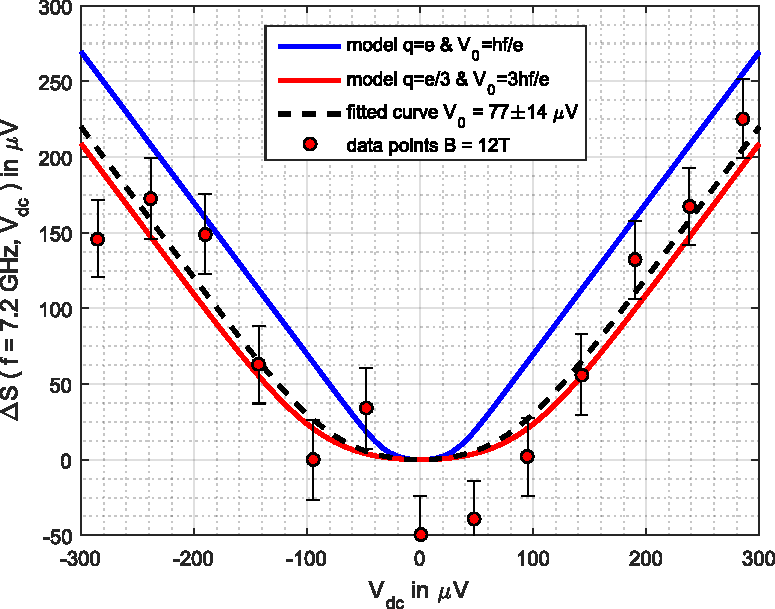
\includegraphics[width = 6.5 cm]{./chap2/nu_2_3_RF_noise_vs_Vdc_at_7_2GHz} &
			& 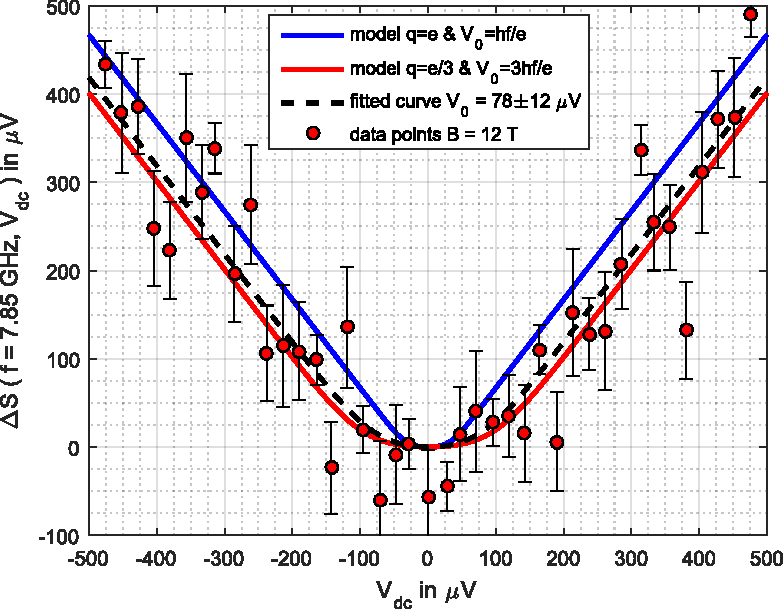
\includegraphics[width = 6.5 cm]{./chap2/nu_2_3_RF_noise_vs_Vdc_at_7_85GHz}
			
		\end{tabular}
	\end{center}
	
	\caption{\textbf{High frequency noise measurement at fractional filling factor $\nu = \frac{2}{3}$.} \textbf{(a)} Few red circle points are measured to show they are closer to the model of fractional charge $q = \frac{e}{3}$ in red line than the blue line corresponding to $q = e$. \textbf{(b)} More points are measured in a wider range of bias voltage $V_{\mathrm{dc}}$. Single points do not allow to distinguish between $q = e$ and $q = \frac{e}{3}$ model, but the dashed fitted line is closer to the $q = \frac{e}{3}$ model.}
	\label{fig: RF charac at 2/3}
\end{figure}

The high frequency measurements are divided in two data sets, which are the two panels of figure Fig. \ref{fig: RF charac at 2/3}.
The axes, which are the noise $\Delta S$ in $\upmu$V as a function of $V_{\mathrm{dc}}$ in $\upmu$V, are the same as in previous results for high frequency noise, and also the represented elements are identical with data points plotted in red circles, models in lines, and fit in dashed lines.
In the panel (a), the measurement is performed at a frequency $f = 7.2$ GHz, with few points, in a medium range of $\pm300 \upmu$V, whereas in the panel (b) the measurement is performed at a close frequency $f = 7.85$ GHz, in a larger range of $\pm500 \upmu$V, with more points.
First one remarks that the error-bars of data points are much bigger than for last subsection results in the integer quantum Hall regime.
This reduction of the measurement sensitivity is due to the decrease of the gain of the measurement line with the magnetic field.
It can have two origins, the increasing impedance mismatch between the sample resistance, which is proportional to the magnetic field, and the lines 50 $\Omega$ impedance, and the increase of noise attenuation in the propagation between the quantum point contact and the output Ohmic contact.
Due to this bigger error-bars, when a lot of points are measured in the panel (b), it is not clear for each single point to determine if they agree with a model of charge $q = e$ or $q = e^{\star} = \frac{e}{3}$.
In the panel (a), with fewer points, the error bars are small enough to have data points consistent with the model \ref{eq: RF noise charge e} with charge $q = \frac{e}{3}$ in red line, and not with charge $q = e$ in blue line.
The fit enables to take into account all points together in the determination of the threshold voltage $V_{0}$, the results in the panel (a) as seen from each individual point show a dashed line close to the model $q = \frac{e}{3}$, and in the panel (b) it enables to conclude because it also gives a dashed line close to the model $q = \frac{e}{3}$.
These measurements by the following equation \ref{eq: RF noise charge e} indicate that in this fractional regime results are the same as in the integer regime with just the elementary charge replaced by fractional one.
In the integer case the absence of noise, meaning the absence of microwave photons emitted at the energy $hf$, when the voltage difference between the two input edge-channels is below the threshold $V_{0} = \frac{hf}{q}$, is due to the Pauli's exclusion principle and the Fermionic statistics of electrons.
Indeed only electrons at energies between the Fermi level of the opposite edge-channel and $eV_{\mathrm{dc}}$ above it, can tunnel through the quantum point contact because other states are fully occupied, so the generated out-of-equilibrium state as a maximum of available energy of $eV_{\mathrm{dc}}$ to generate microwave photons of quantized energy $hf$.
For elementary particles of fractional charge $\frac{e}{3}$ introduced by Laughlin \cite{laughlin1983anomalous}, the expected statistic is an anyonic statistic and not a Fermionic statistic, so the experiment seems to confirm the work \cite{haldane1991fractional} suggesting that there may be an effect analogue to Pauli's exclusion principle for fractional charges.

This experiment has been preceded by several theoretical proposals \cite{crepieux2004photoassisted,ferraro2014multiple,carrega2014finite,carrega2012spectral} aiming at computing the finite frequency shot noise through a tunnel barrier in presence of fractionally charged particles.
%In these works the expected shape of the finite frequency noise present peaks as a function of bias voltage that are not seen in this experiment.
In these works the noise plateau is predicted for voltages $V_{\mathrm{dc}}$ close to zero.
This plateau stops and the noise presents some variation as predicted when the introduced characteristic frequency $f_{J} = \frac{qV_{\mathrm{dc}}}{h}$, with $q$ the fractional charge, is equal to the noise measurement frequency $f$.
Their calculations are based on a Tomonaga-Luttinger liquid model from which all quantities conductance, zero frequency shot noise and finite frequency shot noise are evaluated.
This precise model leads to the presence of noise peaks as a function of $V_{\mathrm{dc}}$ at $f_{J} = f$, which are not observed in this experiment.
Without assuming a Tomonaga-Luttinger liquid model, and without evaluating the conductance and the low frequency shot noise, theoretical calculations \cite{roussel2016perturbative} in the weak-backscattering regime link the conductance and the zero frequency shot noise to finite frequency shot noise.
This correspondence between the finite frequency and zero frequency measurements is only determined by the comparison between the measurement frequency $f$ and the characteristic frequency $f_{J}$.
In the experimental conditions, this link is approximate by equation \eqref{eq: link shot noise 0 and f}.

\begin{equation}
\Delta S\left(f,V_{\mathrm{dc}}\right) = \frac{1}{2}\left(\Delta S\left(0,V_{\mathrm{dc}}-\frac{hf}{q}\right)+\Delta S\left(0,V_{\mathrm{dc}}+\frac{hf}{q}\right)\right) \label{eq: link shot noise 0 and f}
\end{equation}

Since for the chosen transmission $D = 0.8$ the conductance is constant with bias voltage, see panel (b) figure Fig. \ref{fig: LF charac at 2/3}, the zero frequency shot noise is given by equation \eqref{eq: bruit BF nu=2/3}, see panel (d) figure Fig. \ref{fig: LF charac at 2/3}, the finite frequency noise deduced by equations \eqref{eq: bruit BF nu=2/3} and \eqref{eq: link shot noise 0 and f} is given by \eqref{eq: RF noise charge e} , see figure Fig. \ref{fig: RF charac at 2/3}.

\subsubsection*{Noise frequency dependence studied with fractional charges at filling factor $\nu = \frac{4}{3}$}

To study the frequency dependence in the fractional quantum Hall effect, we need to perform more measurements at different frequencies.
As at $\nu = \frac{2}{3}$ the measurement gain is low, the other technique to reach the fractional quantum Hall regime is to adjust the magnetic field for a fractional filling factor above 1.
The chosen filling factor is $\nu = \frac{4}{3}$ reached at $B = 5.7$ T, at this filling factor the measurement gain increase compared to $\nu = \frac{2}{3}$ and the high frequency noise measurement can be repeated for several frequencies from 3.5 GHz to 8 GHz.

\paragraph*{Low frequency characterization.}

\begin{figure}[hptb]
	\begin{center}
		\begin{tabular}{c c c c}
			(a) & & (b) & \\
			& 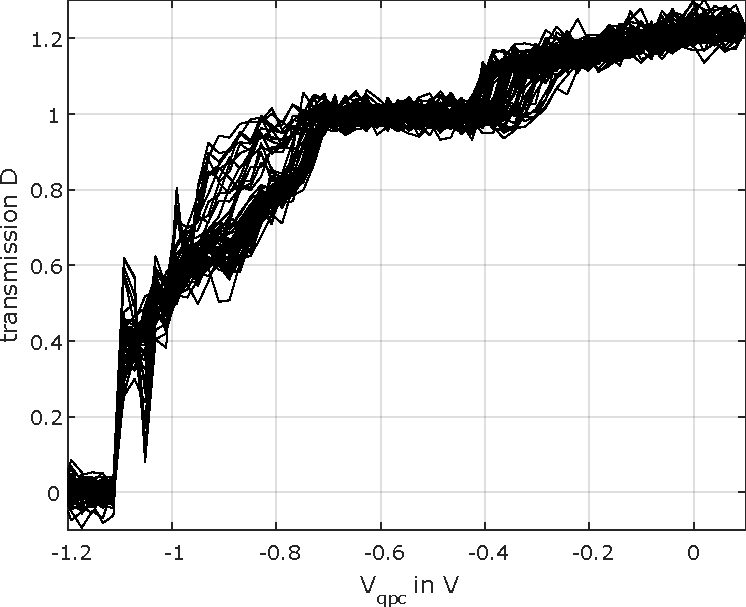
\includegraphics[width = 6.5 cm]{./chap2/nu_4_3_D_vs_Vqpc_for_several_Vdc} &
			& 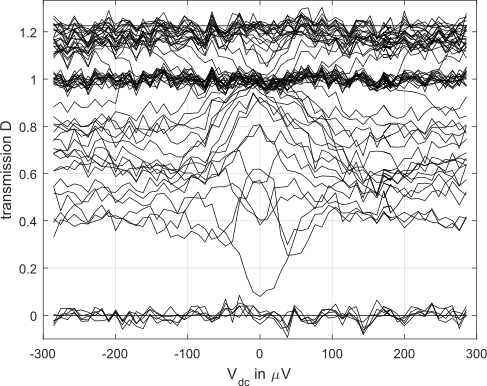
\includegraphics[width = 6.5 cm]{./chap2/nu_4_3_D_vs_Vdc_for_several_Vqpc} \\
			(c) & & (d) & \\
			& \includegraphics[width = 6.5 cm]{./chap2/nu_4_3_noise_vs_D_for_several_Vdc} &
			& 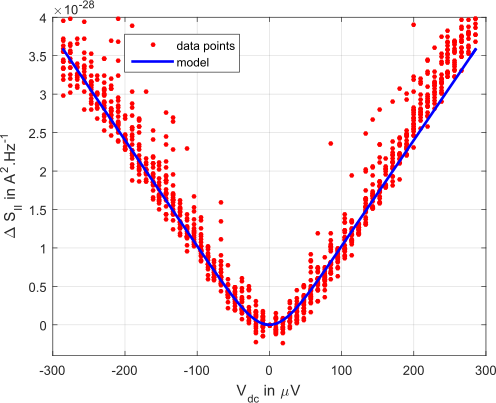
\includegraphics[width = 6.5 cm]{./chap2/nu_4_3_noise_vs_Vdc_for_D_1_15_1_3}
		\end{tabular}
	\end{center}
	
	\caption{\textbf{Conductance and low frequency noise measurement at fractional filling factor $\nu = \frac{4}{3}$.} In this figure the same measures as in figure Fig. \ref{fig: LF charac at 2/3} are plotted. \textbf{(a)} The measurements at different bias voltage of transmission versus gate voltage $V_{\mathrm{qpc}}$ show one step at a conductance of $G = \frac{e^{2}}{h}$ labelled as transmission $D = 1$ and the second step is not fully measured as it saturates before a conductance of $G = \frac{e^{2}}{h}+\frac{e^{2}}{3h}$ corresponding to a transmission of $D = 1+\frac{1}{3}$. \textbf{(b)} The same measurement plotted as a function of the bias voltage show an accumulation of line at the plateau location of transmission 1, and only at a transmission $D = 1.2$ the transmission is independent of $V_{\mathrm{dc}}$, so it is the transmission chosen for the high frequency noise measurement. \textbf{(c)} The noise measurement as a function of the transmission shows two parabolas corresponding to the two equations \eqref{eq: bruit BF nu=4/3}. These two parabolas can be interpreted by the partitioning of two edge-channels of conductance $G = \frac{e^{2}}{h}$ and $G = \frac{e^{2}}{3h}$, and carrying charge $q = e$ and $q = \frac{e}{3}$. \textbf{(d)} Only points at a transmission $D \geq 1.15$ are selected in this graph where the noise is plotted as a function of bias voltage. The blue line is given by the second equation of \eqref{eq: bruit BF nu=4/3} which confirms the model of charge $q = \frac{e}{3}$.
	%The transmission is set at $D = 1.2$ for high frequency noise measurement where the low frequency noise measurement agrees with the blue line model.
	}
	\label{fig: LF charac at 4/3}
\end{figure}

The low frequency measurements in figure Fig. \ref{fig: LF charac at 4/3} show the presence of fractional charges at filling factor $\nu = \frac{4}{3}$.
As previously the panels (a) and (b) display the conductance measurements as a function of gate and bias voltages $V_{\mathrm{qpc}}$ and $V_{\mathrm{dc}}$.
On the panel (a), the conductance shows one clear step at $-0.7$ V$\leq V_{\mathrm{qpc}}\leq -0.4$ V, which corresponds to a transmission $D = 1$, for more negative $V_{\mathrm{qpc}}\leq -1.2$ V the quantum point contact is closed $D = 0$, for more positive value the quantum point contact is not completely open and the transmission saturates at 1.25 before $\frac{4}{3}$.
On the panel (b), the darker zone at $D = 1$ confirms the conductance plateau, the other accumulation of lines around  $D = 1.2$ agrees with saturation of the transmission before the complete opening of the quantum point contact.
The panel (c) still plots the Fano factor defined here as the low frequency noise $\Delta S\left(f=0,V_{\mathrm{dc}}\right)$ divided by $4\frac{e^{2}}{h}k_{\mathrm{B}}T_{\mathrm{elec}}\left(\frac{eV_{\mathrm{dc}}}{2k_{\mathrm{B}}T_{\mathrm{elec}}}\coth\left(\frac{eV_{\mathrm{dc}}}{2k_{\mathrm{B}}T_{\mathrm{elec}}}\right)-1\right)$.
The measured points in red points are consistent with a model in blue line showing a double parabola shape.
This model is based on two edge channels, for transmission $0 \leq D \leq 1$ one edge channel of conductance $\frac{e^{2}}{h}$ and carrying charges $q = e$ is partitioned, for transmission $0 \leq D^{\star} \leq 1$, with $D^{\star} = \frac{D-1}{3}$, the partitioned edge channel has a conductance $\frac{e^{2}}{3h}$ and carries charges $q = e^{\star} = \frac{e}{3}$.
The two parabolas are given by the two equations \eqref{eq: bruit BF nu=4/3}.

\begin{align}
\Delta S\left(f=0,V_{\mathrm{dc}}\right) &= 4D\left(1-D\right)\frac{e^{2}}{h}k_{\mathrm{B}}T_{\mathrm{elec}}\left(\frac{eV_{\mathrm{dc}}}{2k_{\mathrm{B}}T_{\mathrm{elec}}}\coth\left(\frac{eV_{\mathrm{dc}}}{2k_{\mathrm{B}}T_{\mathrm{elec}}}\right)-1\right) \\
\Delta S\left(f=0,V_{\mathrm{dc}}\right) &= 4D^{\star}\left(\frac{1}{3}-D^{\star}\right)\frac{e^{2}}{3h}k_{\mathrm{B}}T_{\mathrm{elec}}\left(\frac{e^{\star}V_{\mathrm{dc}}}{2k_{\mathrm{B}}T_{\mathrm{elec}}}\coth\left(\frac{e^{\star}V_{\mathrm{dc}}}{2k_{\mathrm{B}}T_{\mathrm{elec}}}\right)-1\right)
\label{eq: bruit BF nu=4/3}	
\end{align}

The smallest parabola indicates the presence of fractional charges, which we are interesting in. 
To confirm their presence the panel (d) plots the low frequency shot noise $\Delta S\left(f=0,V_{\mathrm{dc}}\right)$ divided by $D^{\star}\left(1-D^{\star}\right)$ for $0.5 \leq D^{\star}$ as a function of $V_{\mathrm{dc}}$.
As expected the measured red points agree with the blue line model given by the second equation of \eqref{eq: bruit BF nu=4/3}.
In this graph the charge is given by the slope of the noise, and one can remark that its slope is twice smaller than for the $\nu = \frac{2}{3}$ figure Fig. \ref{fig: LF charac at 2/3} panel (d), they have the same charge $q = e^{\star}$ but they have different conductance $\frac{2e^{2}}{3h}$ for $\nu = \frac{2}{3}$ and $\frac{e^{2}}{3h}$ for $\nu = \frac{4}{3}$.
The working point for high frequency measurements is chosen at a transmission $D = 1.2$ thanks to these measurements.

\paragraph*{High frequency measurements.}

\begin{figure}[hptb]
	\begin{center}
		\begin{tabular}{c c c c}
			(a) & & (b) & \\
			& 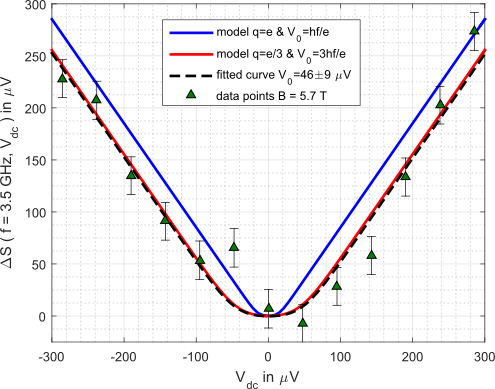
\includegraphics[width = 6.5 cm]{./chap2/nu_4_3_RF_noise_vs_Vdc_at_3_5GHz} &
			& 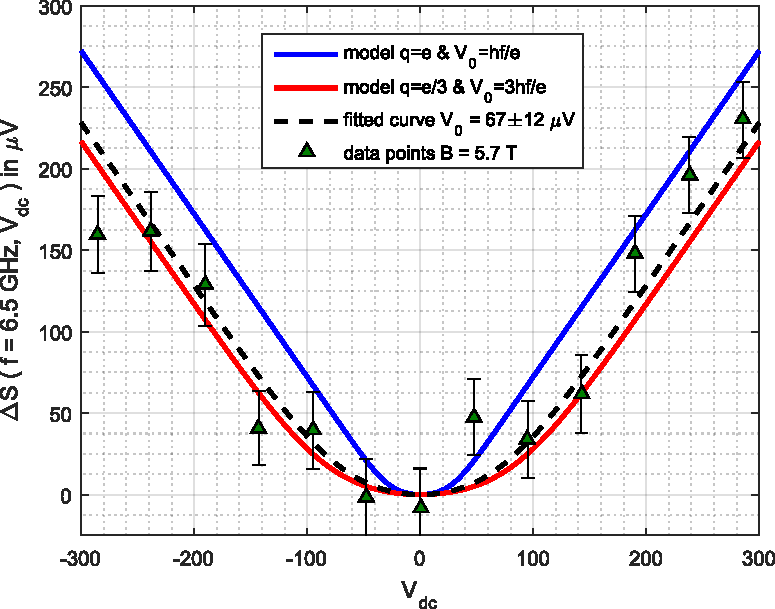
\includegraphics[width = 6.5 cm]{./chap2/nu_4_3_RF_noise_vs_Vdc_at_6_5GHz} \\
			(c) & & (d) & \\
			& 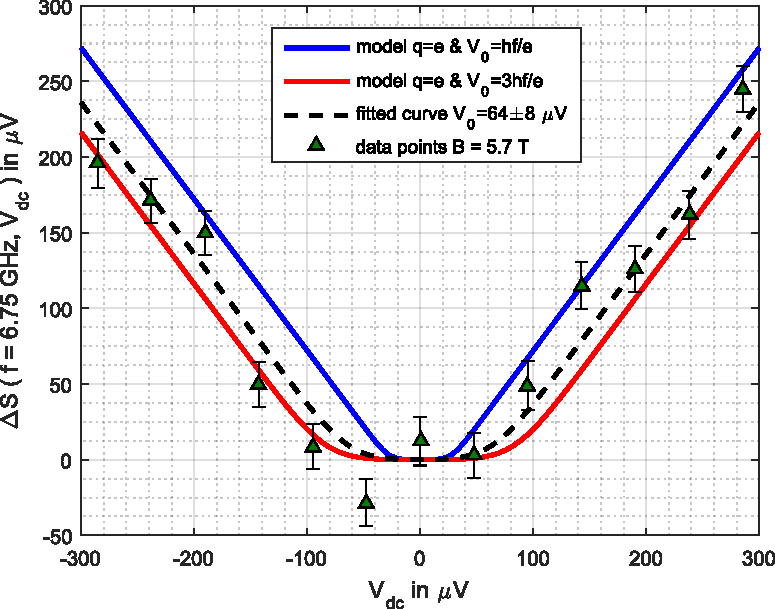
\includegraphics[width = 6.5 cm]{./chap2/nu_4_3_RF_noise_vs_Vdc_at_6_75GHz} &
			& 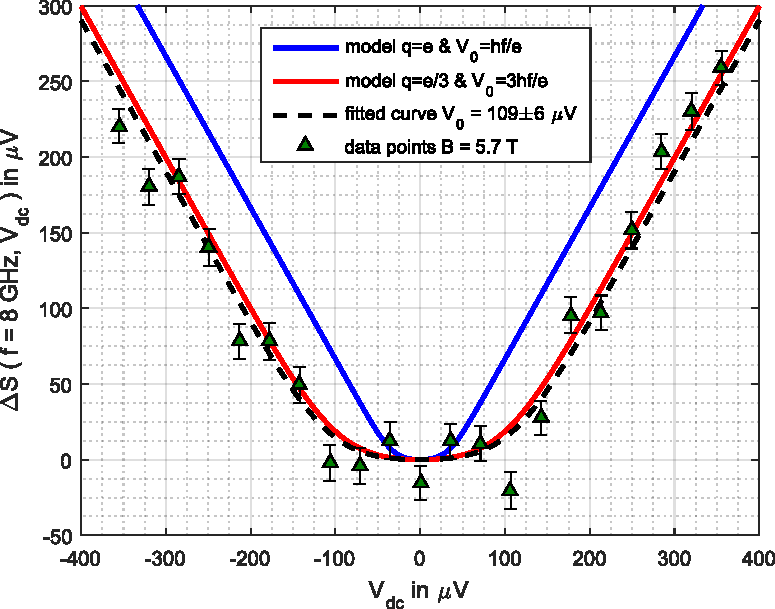
\includegraphics[width = 6.5 cm]{./chap2/nu_4_3_RF_noise_vs_Vdc_at_8GHz}
		\end{tabular}
	\end{center}
	
	\caption{\textbf{High frequency noise measurement for different frequencies between $f= 3.5$ GHz and $f = 8$ GHz at filling factor $\nu = \frac{4}{3}$.} Data points are green triangles for the filling factor $\nu = \frac{4}{3}$. For the chosen weak-backscattering regime data points in all panels and the fitted curve in dashed lines are consistent with the model $q = \frac{e}{3}$ in red line. Between different panels the measurement frequency $f$ is increased from $f = 3.5$ GHz in \textbf{(a)}, $f = 6.5$ GHz in \textbf{(b)}, $f = 6.75$ GHz in \textbf{(c)}, to $f = 8$ GHz in \textbf{(d)}.}
	\label{fig: RF charac at 4/3}
\end{figure}

Following the same method as above the high frequency noise is measured and plotted in green triangles in figure Fig. \ref{fig: RF charac at 4/3}.
The four panels are measurements at increasing frequency from 3.5 GHz to 8 GHz.
In each panel the blue line is the model \eqref{eq: RF noise charge e} with a charge $q = e$, the red line with a charge $q = \frac{e}{3}$, and the dashed line is the result of threshold voltage $V_{0}$ fit in equation \eqref{eq: fit RF noise}.
In the four panels data points and the fitted dashed lines are closer to the red line than the blue line.
From the high frequency noise, we can also conclude that excitations are carried by fractional charges at the transmission $D = 1.2$ and filling factor $\nu = \frac{4}{3}$.
This conclusion is valid for each panel, so for each frequency, and one can remark that the voltage threshold $V_{0}$ increases from  $46 \pm 9$ $\upmu$V at 3.5 GHz to $109 \pm 6$ $\upmu$V at 8 GHz.
With these measurements and the high frequency noise measurement at filling factor $\nu = 3$, there are two data sets, which allow to study the evolution of the high frequency noise with the measurement frequency.

\subsection{Frequency and charge dependence}

\begin{figure}[hptb]
	\begin{center}
		\begin{tabular}{c c c c}
			(a) & & (b) & \\
			& 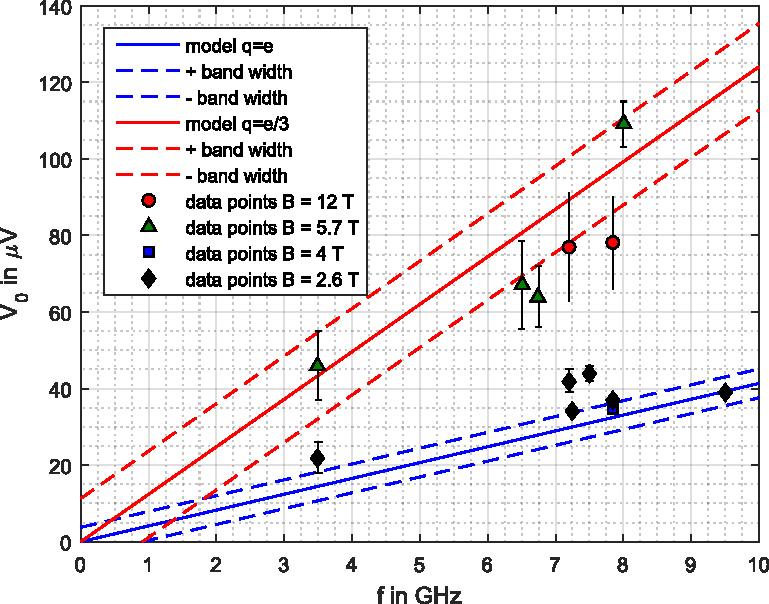
\includegraphics[width = 6.5 cm]{./chap2/V_0_vs_f_for_different_nu} &
			& 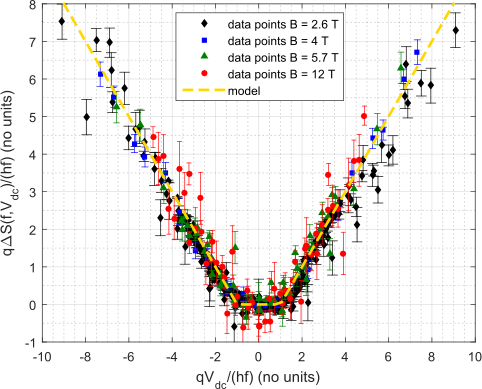
\includegraphics[width = 6.5 cm]{./chap2/noise_vs_V_dc_for_different_nu}
		\end{tabular}
	\end{center}
	
	\caption{\textbf{Frequency and charge dependence of high frequency noise.} \textbf{(a)} The threshold voltage $V_{0}$ got from the fitting of experimental data is plotted as a function of the measurement frequency. The shape and the colour of points correspond to the same shape and colour for the filling factor of the measurement points. The red line is the threshold voltage given by a model of fractional charge $q = \frac{e}{3}$ in equation \eqref{eq: Josephson relation}. The blue line is the model for an integer charge $q = e$. Dashed lines are similar to plain lines with a frequency $f$ shifted by plus or minus the measurement bandwidth around $f$. \textbf{(b)} All high frequency noise measurements $\Delta S$ plotted as a function of the bias voltage $V_{\mathrm{dc}}$. Both noise and voltage are multiplied by the factor $\frac{q}{hf}$ with $f$ the measurement frequency and $q$ the measured charge $e$ or $\frac{e}{3}$ given in (a). All data are consistent with the same model \eqref{eq: RF noise charge e} in yellow dashed line.}
	\label{fig: charac for all nu}
\end{figure}

This subsection re-use all measurements at different filling factors and different frequencies to discuss the charge and frequency dependence of the high frequency noise.
The voltage threshold $V_{0}$ is the fitting parameter used to determine the charge in the different measurements, so it is the parameter that summarizes the high frequency noise measurement at one frequency and one filling factor.
The equation \eqref{eq: Josephson relation} relates the measured threshold voltage $V_{0}$ with the chosen measurement frequency $f$ and the excitations charge $q$.
The panel (a) of figure Fig. \ref{fig: charac for all nu} checks the agreement between measurements and relation \eqref{eq: Josephson relation}.
%The characteristic frequency associated with the threshold voltage $\frac{eV_{0}}{h}$ is plotted as a function of the measurement frequency $f$.
The threshold voltage $\frac{eV_{0}}{h}$ is plotted as a function of the measurement frequency $f$.
The data points have the same shape and colour as above associated with their filling factor: red circle for $\nu = \frac{2}{3}$, green triangles for $\nu = \frac{4}{3}$, blue squares for $\nu = 2$, black diamonds for $\nu = 3$.
The blue line is the equation \eqref{eq: Josephson relation} with integer charge $q = e$ and the red line with fractional charge $q = \frac{e}{3}$.
The data points at integer filling factors follow the trend of integer charge blue line, and the data points at fractional filling factor follow the trend of fractional charge red line.
To get a better agreement between data points and the models, one needs to consider that the high frequency noise is integrated on a bandwidth around the central frequency $f$.
This integration increases only the signal level and the effective electronic temperature $T_{\mathrm{elec}}$ when the band width increases if the noise measurement gain is flat with frequency.
This effect is already taken into account, but if the noise measurement gain is not flat with frequency there are more modifications of the noise measurement parameters.
With a gain that depends on frequency, the effective central frequency $f$ at which the noise is measured can be shifted inside the bandwidth $\Delta f$, so the dashed line are the models given by \eqref{eq: Josephson relation}, with a frequency $f$ replaced by $f\pm\frac{\Delta f}{\sqrt{3}}$.
The blue and red dashed lines are still well separate, this allows separating integer and fractional charges, and most of the data points error bars overlap the interval between the two dashed lines of either one model or the other. 
The threshold voltage $V_{0}$ of noise emission at frequency $f$ is quantitatively described by the relation \eqref{eq: Josephson relation} in the integer and in the fractional quantum Hall effect, with the additional condition of a quantum point contact in the weak backscattering regime for fractional quantum Hall effect.
After experimentally establishing the frequency and charge evolution of the threshold voltage, we can discuss the shape of the noise as a function of the bias voltage $V_{\mathrm{dc}}$.
To compare the different results, the bias voltage $V_{\mathrm{dc}}$ is divided by the associated theoretical threshold voltage $\frac{hf}{q}$, and the high frequency noise $\Delta S\left(f,V_{\mathrm{dc}}\right)$ is also divided by the same voltage, since it is also measured in $\upmu$V.
The panel (b) of figure Fig. \ref{fig: charac for all nu} gathers all the rescale high frequency noise data points for all filling factors and frequencies and keeps the same colour and shape code for data points.
All these data points are distributed along the model in yellow dashed line of equation \eqref{eq: general finite freq noise},

\begin{equation}
y = \frac{x+1}{2}\coth\left(\frac{x+1}{2}\right)+\frac{x-1}{2}\coth\left(\frac{x-1}{2}\right)-\coth\left(\frac{1}{2}\right) \label{eq: general finite freq noise}
\end{equation}

with $y = \frac{q\Delta S\left(f,V_{\mathrm{dc}}\right)}{hf}$ and $x = \frac{qV_{\mathrm{dc}}}{hf}$.
All the high frequency noise curve is just rescaled by the frequency of measurement and the excitations charge, and keeps the same shape as a function of $V_{\mathrm{dc}}$.
The voltage rescale is given by only by the measurement frequency $f$ and the charge $q$, it provides a direct measurement of fractional charges without the necessity of gain calibration.




